\documentclass[twoside]{book}

% Packages required by doxygen
\usepackage{fixltx2e}
\usepackage{calc}
\usepackage{doxygen}
\usepackage[export]{adjustbox} % also loads graphicx
\usepackage{graphicx}
\usepackage[utf8]{inputenc}
\usepackage{makeidx}
\usepackage{multicol}
\usepackage{multirow}
\PassOptionsToPackage{warn}{textcomp}
\usepackage{textcomp}
\usepackage[nointegrals]{wasysym}
\usepackage[table]{xcolor}

% Font selection
\usepackage[T1]{fontenc}
\usepackage[scaled=.90]{helvet}
\usepackage{courier}
\usepackage{amssymb}
\usepackage{sectsty}
\renewcommand{\familydefault}{\sfdefault}
\allsectionsfont{%
  \fontseries{bc}\selectfont%
  \color{darkgray}%
}
\renewcommand{\DoxyLabelFont}{%
  \fontseries{bc}\selectfont%
  \color{darkgray}%
}
\newcommand{\+}{\discretionary{\mbox{\scriptsize$\hookleftarrow$}}{}{}}

% Page & text layout
\usepackage{geometry}
\geometry{%
  a4paper,%
  top=2.5cm,%
  bottom=2.5cm,%
  left=2.5cm,%
  right=2.5cm%
}
\tolerance=750
\hfuzz=15pt
\hbadness=750
\setlength{\emergencystretch}{15pt}
\setlength{\parindent}{0cm}
\setlength{\parskip}{3ex plus 2ex minus 2ex}
\makeatletter
\renewcommand{\paragraph}{%
  \@startsection{paragraph}{4}{0ex}{-1.0ex}{1.0ex}{%
    \normalfont\normalsize\bfseries\SS@parafont%
  }%
}
\renewcommand{\subparagraph}{%
  \@startsection{subparagraph}{5}{0ex}{-1.0ex}{1.0ex}{%
    \normalfont\normalsize\bfseries\SS@subparafont%
  }%
}
\makeatother

% Headers & footers
\usepackage{fancyhdr}
\pagestyle{fancyplain}
\fancyhead[LE]{\fancyplain{}{\bfseries\thepage}}
\fancyhead[CE]{\fancyplain{}{}}
\fancyhead[RE]{\fancyplain{}{\bfseries\leftmark}}
\fancyhead[LO]{\fancyplain{}{\bfseries\rightmark}}
\fancyhead[CO]{\fancyplain{}{}}
\fancyhead[RO]{\fancyplain{}{\bfseries\thepage}}
\fancyfoot[LE]{\fancyplain{}{}}
\fancyfoot[CE]{\fancyplain{}{}}
\fancyfoot[RE]{\fancyplain{}{\bfseries\scriptsize Generated by Doxygen }}
\fancyfoot[LO]{\fancyplain{}{\bfseries\scriptsize Generated by Doxygen }}
\fancyfoot[CO]{\fancyplain{}{}}
\fancyfoot[RO]{\fancyplain{}{}}
\renewcommand{\footrulewidth}{0.4pt}
\renewcommand{\chaptermark}[1]{%
  \markboth{#1}{}%
}
\renewcommand{\sectionmark}[1]{%
  \markright{\thesection\ #1}%
}

% Indices & bibliography
\usepackage{natbib}
\usepackage[titles]{tocloft}
\setcounter{tocdepth}{3}
\setcounter{secnumdepth}{5}
\makeindex

% Hyperlinks (required, but should be loaded last)
\usepackage{ifpdf}
\ifpdf
  \usepackage[pdftex,pagebackref=true]{hyperref}
\else
  \usepackage[ps2pdf,pagebackref=true]{hyperref}
\fi
\hypersetup{%
  colorlinks=true,%
  linkcolor=blue,%
  citecolor=blue,%
  unicode%
}

% Custom commands
\newcommand{\clearemptydoublepage}{%
  \newpage{\pagestyle{empty}\cleardoublepage}%
}

\usepackage{caption}
\captionsetup{labelsep=space,justification=centering,font={bf},singlelinecheck=off,skip=4pt,position=top}

%===== C O N T E N T S =====

\begin{document}

% Titlepage & ToC
\hypersetup{pageanchor=false,
             bookmarksnumbered=true,
             pdfencoding=unicode
            }
\pagenumbering{roman}
\begin{titlepage}
\vspace*{7cm}
\begin{center}%
{\Large My Project }\\
\vspace*{1cm}
{\large Generated by Doxygen 1.8.11}\\
\end{center}
\end{titlepage}
\clearemptydoublepage
\tableofcontents
\clearemptydoublepage
\pagenumbering{arabic}
\hypersetup{pageanchor=true}

%--- Begin generated contents ---
\chapter{Namespace Index}
\section{Namespace List}
Here is a list of all documented namespaces with brief descriptions\+:\begin{DoxyCompactList}
\item\contentsline{section}{\hyperlink{namespaceed}{ed} \\*Espacio de nombres ED }{\pageref{namespaceed}}{}
\end{DoxyCompactList}

\chapter{Hierarchical Index}
\section{Class Hierarchy}
This inheritance list is sorted roughly, but not completely, alphabetically\+:\begin{DoxyCompactList}
\item \contentsline{section}{ed\+:\+:Donante\+Interfaz}{\pageref{classed_1_1DonanteInterfaz}}{}
\begin{DoxyCompactList}
\item \contentsline{section}{ed\+:\+:Donante}{\pageref{classed_1_1Donante}}{}
\end{DoxyCompactList}
\item \contentsline{section}{ed\+:\+:Monticulo\+Interfaz}{\pageref{classed_1_1MonticuloInterfaz}}{}
\begin{DoxyCompactList}
\item \contentsline{section}{ed\+:\+:Monticulo}{\pageref{classed_1_1Monticulo}}{}
\end{DoxyCompactList}
\end{DoxyCompactList}

\chapter{Class Index}
\section{Class List}
Here are the classes, structs, unions and interfaces with brief descriptions\+:\begin{DoxyCompactList}
\item\contentsline{section}{\hyperlink{classed_1_1Monomio}{ed\+::\+Monomio} \\*Clase \hyperlink{classed_1_1Monomio}{Monomio} hereda de \hyperlink{classed_1_1MonomioInterfaz}{Monomio\+Interfaz} }{\pageref{classed_1_1Monomio}}{}
\item\contentsline{section}{\hyperlink{classed_1_1MonomioInterfaz}{ed\+::\+Monomio\+Interfaz} }{\pageref{classed_1_1MonomioInterfaz}}{}
\item\contentsline{section}{\hyperlink{classed_1_1Polinomio}{ed\+::\+Polinomio} \\*Clase \hyperlink{classed_1_1Polinomio}{Polinomio} hereda de \hyperlink{classed_1_1PolinomioInterfaz}{Polinomio\+Interfaz} }{\pageref{classed_1_1Polinomio}}{}
\item\contentsline{section}{\hyperlink{classed_1_1PolinomioInterfaz}{ed\+::\+Polinomio\+Interfaz} }{\pageref{classed_1_1PolinomioInterfaz}}{}
\end{DoxyCompactList}

\chapter{File Index}
\section{File List}
Here is a list of all documented files with brief descriptions\+:\begin{DoxyCompactList}
\item\contentsline{section}{includes/\hyperlink{colors_8hpp}{colors.\+hpp} \\*Colores para la terminal }{\pageref{colors_8hpp}}{}
\item\contentsline{section}{includes/\hyperlink{funciones_8hpp}{funciones.\+hpp} \\*Fichero de funciones que utilizan el grafo }{\pageref{funciones_8hpp}}{}
\item\contentsline{section}{includes/\hyperlink{Grafo_8hpp}{Grafo.\+hpp} \\*Clase Grafo }{\pageref{Grafo_8hpp}}{}
\item\contentsline{section}{includes/\hyperlink{librerias_8hpp}{librerias.\+hpp} \\*Librerias incluidas en los hpp }{\pageref{librerias_8hpp}}{}
\item\contentsline{section}{includes/\hyperlink{macros_8hpp}{macros.\+hpp} \\*Macros para el diseño de pantallas }{\pageref{macros_8hpp}}{}
\item\contentsline{section}{includes/\hyperlink{Vertice_8hpp}{Vertice.\+hpp} \\*Clase Vertice }{\pageref{Vertice_8hpp}}{}
\item\contentsline{section}{src/\hyperlink{main_8cpp}{main.\+cpp} \\*Funcion Main del programa }{\pageref{main_8cpp}}{}
\end{DoxyCompactList}

\chapter{Namespace Documentation}
\hypertarget{namespaceed}{}\section{ed Namespace Reference}
\label{namespaceed}\index{ed@{ed}}


Espacio de nombres ED.  


\subsection*{Classes}
\begin{DoxyCompactItemize}
\item 
class \hyperlink{classed_1_1Donante}{Donante}
\begin{DoxyCompactList}\small\item\em Clase \hyperlink{classed_1_1Donante}{Donante}. \end{DoxyCompactList}\item 
class \hyperlink{classed_1_1DonanteInterfaz}{Donante\+Interfaz}
\begin{DoxyCompactList}\small\item\em Clase \hyperlink{classed_1_1DonanteInterfaz}{Donante\+Interfaz} usada por \hyperlink{classed_1_1Donante}{Donante}. \end{DoxyCompactList}\item 
class \hyperlink{classed_1_1Monticulo}{Monticulo}
\begin{DoxyCompactList}\small\item\em Clase \hyperlink{classed_1_1Monticulo}{Monticulo}. \end{DoxyCompactList}\item 
class \hyperlink{classed_1_1MonticuloInterfaz}{Monticulo\+Interfaz}
\begin{DoxyCompactList}\small\item\em Clase \hyperlink{classed_1_1MonticuloInterfaz}{Monticulo\+Interfaz}. \end{DoxyCompactList}\end{DoxyCompactItemize}


\subsection{Detailed Description}
Espacio de nombres ED. 

Espacio de nombres ed. 
\chapter{Class Documentation}
\hypertarget{classed_1_1Donante}{}\section{ed\+:\+:Donante Class Reference}
\label{classed_1_1Donante}\index{ed\+::\+Donante@{ed\+::\+Donante}}


Clase \hyperlink{classed_1_1Donante}{Donante}.  




{\ttfamily \#include $<$Donante.\+hpp$>$}



Inheritance diagram for ed\+:\+:Donante\+:\nopagebreak
\begin{figure}[H]
\begin{center}
\leavevmode
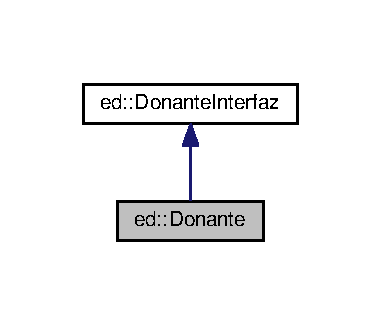
\includegraphics[width=183pt]{classed_1_1Donante__inherit__graph}
\end{center}
\end{figure}


Collaboration diagram for ed\+:\+:Donante\+:\nopagebreak
\begin{figure}[H]
\begin{center}
\leavevmode
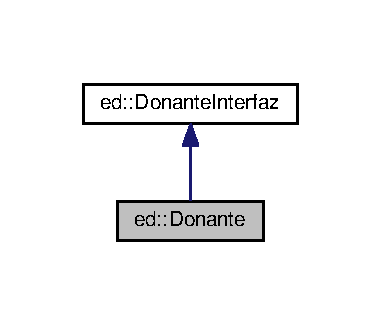
\includegraphics[width=183pt]{classed_1_1Donante__coll__graph}
\end{center}
\end{figure}
\subsection*{Public Member Functions}
\begin{Indent}{\bf Constructores}\par
\begin{DoxyCompactItemize}
\item 
{\bfseries Donante} ()\hypertarget{classed_1_1Donante_a2847e02d165f0850b1917b739e2ef68a}{}\label{classed_1_1Donante_a2847e02d165f0850b1917b739e2ef68a}

\item 
{\bfseries Donante} (std\+::string Name, std\+::string Second\+Name, std\+::string Group, bool RH)\hypertarget{classed_1_1Donante_adbdccfbaed5d68439b52b277bb6ea6d3}{}\label{classed_1_1Donante_adbdccfbaed5d68439b52b277bb6ea6d3}

\item 
{\bfseries Donante} (const \hyperlink{classed_1_1Donante}{Donante} \&don)\hypertarget{classed_1_1Donante_ac2f8da906fe62462be028e2c7ec4ba48}{}\label{classed_1_1Donante_ac2f8da906fe62462be028e2c7ec4ba48}

\end{DoxyCompactItemize}
\end{Indent}
\begin{Indent}{\bf Observadores}\par
\begin{DoxyCompactItemize}
\item 
std\+::string \hyperlink{classed_1_1Donante_ae76f1220582f41d257d2f91f7addc858}{get\+Name} () const 
\begin{DoxyCompactList}\small\item\em Devuelve el nombre del \hyperlink{classed_1_1Donante}{Donante}. \end{DoxyCompactList}\item 
std\+::string \hyperlink{classed_1_1Donante_ace0406348e755517d3e80ceff18a2f59}{get\+Second\+Name} () const 
\begin{DoxyCompactList}\small\item\em Devuelve el apellido del \hyperlink{classed_1_1Donante}{Donante}. \end{DoxyCompactList}\item 
std\+::string \hyperlink{classed_1_1Donante_a0b1e59193e6c887a7232d48b71bfae33}{get\+Group} () const 
\begin{DoxyCompactList}\small\item\em Devuelve el grupo del \hyperlink{classed_1_1Donante}{Donante}. \end{DoxyCompactList}\item 
bool \hyperlink{classed_1_1Donante_aed957d321e76a3a907849d4cf0f438ee}{get\+RH} () const 
\begin{DoxyCompactList}\small\item\em Devuelve el factor RH del \hyperlink{classed_1_1Donante}{Donante}. \end{DoxyCompactList}\item 
int \hyperlink{classed_1_1Donante_ae0255405dc76a90d2ea383cd8abd4d43}{get\+Donaciones} () const 
\begin{DoxyCompactList}\small\item\em Devuelve el numero de donaciones realizadas por el donante. \end{DoxyCompactList}\end{DoxyCompactItemize}
\end{Indent}
\begin{Indent}{\bf Modificadores}\par
\begin{DoxyCompactItemize}
\item 
void \hyperlink{classed_1_1Donante_a149c2f94803ea99ca0d322e1f54eb3e9}{set\+Name} (const std\+::string \&Name)
\begin{DoxyCompactList}\small\item\em Establece como nombre el string pasado por parametro. \end{DoxyCompactList}\item 
void \hyperlink{classed_1_1Donante_a28b1027f7ceddd66a48a5aad0ead0c43}{set\+Second\+Name} (const std\+::string \&Second\+Name)
\begin{DoxyCompactList}\small\item\em Establece como apellido el string pasado por parametro. \end{DoxyCompactList}\item 
void \hyperlink{classed_1_1Donante_a8e8d2ac356b88e9a83b6a3a573eb76af}{set\+Group} (const std\+::string \&Group)
\begin{DoxyCompactList}\small\item\em Establece como grupo Sanguineo el string pasado por parametro. \end{DoxyCompactList}\item 
void \hyperlink{classed_1_1Donante_ae0c5eed15e7f42de44bde8405e92f598}{set\+RH} (const bool \&RH)
\begin{DoxyCompactList}\small\item\em Establece como apellido el string pasado por parametro. \end{DoxyCompactList}\item 
void {\bfseries set\+Donaciones} (const int \&donaciones)\hypertarget{classed_1_1Donante_a93159ec1442d245ca6d7415e05b9ef3d}{}\label{classed_1_1Donante_a93159ec1442d245ca6d7415e05b9ef3d}

\end{DoxyCompactItemize}
\end{Indent}
\begin{Indent}{\bf Otras funciones de la clase}\par
\begin{DoxyCompactItemize}
\item 
void \hyperlink{classed_1_1Donante_a9d38e1caacf3dee07477fb49da65d65e}{write\+Donante} ()\hypertarget{classed_1_1Donante_a9d38e1caacf3dee07477fb49da65d65e}{}\label{classed_1_1Donante_a9d38e1caacf3dee07477fb49da65d65e}

\begin{DoxyCompactList}\small\item\em Escribe por pantalla la informacion del \hyperlink{classed_1_1Donante}{Donante}. \end{DoxyCompactList}\item 
void \hyperlink{classed_1_1Donante_a82deb00969394d9b5c85c36c3256d4d4}{read\+Donante} ()\hypertarget{classed_1_1Donante_a82deb00969394d9b5c85c36c3256d4d4}{}\label{classed_1_1Donante_a82deb00969394d9b5c85c36c3256d4d4}

\begin{DoxyCompactList}\small\item\em Lee por pantalla la informacion del \hyperlink{classed_1_1Donante}{Donante}. \end{DoxyCompactList}\item 
void \hyperlink{classed_1_1Donante_a86a221eec5fc5800f51a96d732c80124}{modify} ()\hypertarget{classed_1_1Donante_a86a221eec5fc5800f51a96d732c80124}{}\label{classed_1_1Donante_a86a221eec5fc5800f51a96d732c80124}

\begin{DoxyCompactList}\small\item\em Modificar los datos de un donante. \end{DoxyCompactList}\end{DoxyCompactItemize}
\end{Indent}
\begin{Indent}{\bf Sobrecarga de operadores}\par
\begin{DoxyCompactItemize}
\item 
\hyperlink{classed_1_1Donante}{Donante} \& \hyperlink{classed_1_1Donante_ac517a0b7d0110ded5730241ca1357c1b}{operator=} (\hyperlink{classed_1_1Donante}{Donante} don)
\begin{DoxyCompactList}\small\item\em Sobrecarga del operador =. \end{DoxyCompactList}\item 
bool \hyperlink{classed_1_1Donante_a4335aaf566fe258aa97dbe83becc45a0}{operator==} (const \hyperlink{classed_1_1Donante}{Donante} \&don1)
\begin{DoxyCompactList}\small\item\em Devuelve true si ambos donantes son iguales. \end{DoxyCompactList}\item 
bool \hyperlink{classed_1_1Donante_aa6c68c52b4e36454fae3fc252904fb7a}{operator$<$=} (const \hyperlink{classed_1_1Donante}{Donante} \&don1)
\begin{DoxyCompactList}\small\item\em Operador $<$=, nos sera util para el ordenado alfabetico. \end{DoxyCompactList}\item 
bool \hyperlink{classed_1_1Donante_a55423d33ae333c344b079eadf71d1cbe}{operator$>$=} (const \hyperlink{classed_1_1Donante}{Donante} \&don1)
\begin{DoxyCompactList}\small\item\em Operador $>$=, nos sera util para el ordenado en la lista. \end{DoxyCompactList}\end{DoxyCompactItemize}
\end{Indent}
\subsection*{Friends}
\begin{Indent}{\bf Funciones amigas}\par
\begin{DoxyCompactItemize}
\item 
std\+::istream \& \hyperlink{classed_1_1Donante_acbd1fb64ad57f44d7c558c5035f5792a}{operator$>$$>$} (std\+::istream \&stream, \hyperlink{classed_1_1Donante}{Donante} \&d)
\begin{DoxyCompactList}\small\item\em Sobrecarga del operador $>$$>$ \end{DoxyCompactList}\item 
std\+::ostream \& \hyperlink{classed_1_1Donante_ab52eb93adf74c23cd988ea8868a08fa0}{operator$<$$<$} (std\+::ostream \&stream, \hyperlink{classed_1_1Donante}{Donante} const \&d)
\begin{DoxyCompactList}\small\item\em Sobrecarga del operador $<$$<$. \end{DoxyCompactList}\end{DoxyCompactItemize}
\end{Indent}


\subsection{Detailed Description}
Clase \hyperlink{classed_1_1Donante}{Donante}. 

\subsection{Member Function Documentation}
\index{ed\+::\+Donante@{ed\+::\+Donante}!get\+Donaciones@{get\+Donaciones}}
\index{get\+Donaciones@{get\+Donaciones}!ed\+::\+Donante@{ed\+::\+Donante}}
\subsubsection[{\texorpdfstring{get\+Donaciones() const }{getDonaciones() const }}]{\setlength{\rightskip}{0pt plus 5cm}int ed\+::\+Donante\+::get\+Donaciones (
\begin{DoxyParamCaption}
{}
\end{DoxyParamCaption}
) const\hspace{0.3cm}{\ttfamily [inline]}, {\ttfamily [virtual]}}\hypertarget{classed_1_1Donante_ae0255405dc76a90d2ea383cd8abd4d43}{}\label{classed_1_1Donante_ae0255405dc76a90d2ea383cd8abd4d43}


Devuelve el numero de donaciones realizadas por el donante. 

\begin{DoxyReturn}{Returns}
int 
\end{DoxyReturn}


Implements \hyperlink{classed_1_1DonanteInterfaz_a0e72966c68cab8ccb8da1c493a3a6f56}{ed\+::\+Donante\+Interfaz}.

\index{ed\+::\+Donante@{ed\+::\+Donante}!get\+Group@{get\+Group}}
\index{get\+Group@{get\+Group}!ed\+::\+Donante@{ed\+::\+Donante}}
\subsubsection[{\texorpdfstring{get\+Group() const }{getGroup() const }}]{\setlength{\rightskip}{0pt plus 5cm}std\+::string ed\+::\+Donante\+::get\+Group (
\begin{DoxyParamCaption}
{}
\end{DoxyParamCaption}
) const\hspace{0.3cm}{\ttfamily [inline]}, {\ttfamily [virtual]}}\hypertarget{classed_1_1Donante_a0b1e59193e6c887a7232d48b71bfae33}{}\label{classed_1_1Donante_a0b1e59193e6c887a7232d48b71bfae33}


Devuelve el grupo del \hyperlink{classed_1_1Donante}{Donante}. 

\begin{DoxyReturn}{Returns}
String, grupo del donante 
\end{DoxyReturn}


Implements \hyperlink{classed_1_1DonanteInterfaz_a094e88f0c9cd5c7391d5c06a09a667a1}{ed\+::\+Donante\+Interfaz}.

\index{ed\+::\+Donante@{ed\+::\+Donante}!get\+Name@{get\+Name}}
\index{get\+Name@{get\+Name}!ed\+::\+Donante@{ed\+::\+Donante}}
\subsubsection[{\texorpdfstring{get\+Name() const }{getName() const }}]{\setlength{\rightskip}{0pt plus 5cm}std\+::string ed\+::\+Donante\+::get\+Name (
\begin{DoxyParamCaption}
{}
\end{DoxyParamCaption}
) const\hspace{0.3cm}{\ttfamily [inline]}, {\ttfamily [virtual]}}\hypertarget{classed_1_1Donante_ae76f1220582f41d257d2f91f7addc858}{}\label{classed_1_1Donante_ae76f1220582f41d257d2f91f7addc858}


Devuelve el nombre del \hyperlink{classed_1_1Donante}{Donante}. 

\begin{DoxyReturn}{Returns}
String, nombre del donante 
\end{DoxyReturn}


Implements \hyperlink{classed_1_1DonanteInterfaz_acc116c503c26b5dee7c8982e56e5cd59}{ed\+::\+Donante\+Interfaz}.

\index{ed\+::\+Donante@{ed\+::\+Donante}!get\+RH@{get\+RH}}
\index{get\+RH@{get\+RH}!ed\+::\+Donante@{ed\+::\+Donante}}
\subsubsection[{\texorpdfstring{get\+R\+H() const }{getRH() const }}]{\setlength{\rightskip}{0pt plus 5cm}bool ed\+::\+Donante\+::get\+RH (
\begin{DoxyParamCaption}
{}
\end{DoxyParamCaption}
) const\hspace{0.3cm}{\ttfamily [inline]}, {\ttfamily [virtual]}}\hypertarget{classed_1_1Donante_aed957d321e76a3a907849d4cf0f438ee}{}\label{classed_1_1Donante_aed957d321e76a3a907849d4cf0f438ee}


Devuelve el factor RH del \hyperlink{classed_1_1Donante}{Donante}. 

\begin{DoxyReturn}{Returns}
Bool, factor RH del donante 
\end{DoxyReturn}


Implements \hyperlink{classed_1_1DonanteInterfaz_a3607867d874ea4fe71813acb41a0b0ef}{ed\+::\+Donante\+Interfaz}.

\index{ed\+::\+Donante@{ed\+::\+Donante}!get\+Second\+Name@{get\+Second\+Name}}
\index{get\+Second\+Name@{get\+Second\+Name}!ed\+::\+Donante@{ed\+::\+Donante}}
\subsubsection[{\texorpdfstring{get\+Second\+Name() const }{getSecondName() const }}]{\setlength{\rightskip}{0pt plus 5cm}std\+::string ed\+::\+Donante\+::get\+Second\+Name (
\begin{DoxyParamCaption}
{}
\end{DoxyParamCaption}
) const\hspace{0.3cm}{\ttfamily [inline]}, {\ttfamily [virtual]}}\hypertarget{classed_1_1Donante_ace0406348e755517d3e80ceff18a2f59}{}\label{classed_1_1Donante_ace0406348e755517d3e80ceff18a2f59}


Devuelve el apellido del \hyperlink{classed_1_1Donante}{Donante}. 

\begin{DoxyReturn}{Returns}
String, apellido del donante 
\end{DoxyReturn}


Implements \hyperlink{classed_1_1DonanteInterfaz_ad00f542962f6585da7b465c48e65a6e9}{ed\+::\+Donante\+Interfaz}.

\index{ed\+::\+Donante@{ed\+::\+Donante}!operator$<$=@{operator$<$=}}
\index{operator$<$=@{operator$<$=}!ed\+::\+Donante@{ed\+::\+Donante}}
\subsubsection[{\texorpdfstring{operator$<$=(const Donante \&don1)}{operator<=(const Donante &don1)}}]{\setlength{\rightskip}{0pt plus 5cm}bool ed\+::\+Donante\+::operator$<$= (
\begin{DoxyParamCaption}
\item[{const {\bf Donante} \&}]{don1}
\end{DoxyParamCaption}
)\hspace{0.3cm}{\ttfamily [inline]}}\hypertarget{classed_1_1Donante_aa6c68c52b4e36454fae3fc252904fb7a}{}\label{classed_1_1Donante_aa6c68c52b4e36454fae3fc252904fb7a}


Operador $<$=, nos sera util para el ordenado alfabetico. 


\begin{DoxyParams}{Parameters}
{\em const} & \hyperlink{classed_1_1Donante}{Donante}\& don1 \\
\hline
\end{DoxyParams}
\begin{DoxyReturn}{Returns}
bool si $<$= por apellidos 
\end{DoxyReturn}
\index{ed\+::\+Donante@{ed\+::\+Donante}!operator=@{operator=}}
\index{operator=@{operator=}!ed\+::\+Donante@{ed\+::\+Donante}}
\subsubsection[{\texorpdfstring{operator=(\+Donante don)}{operator=(Donante don)}}]{\setlength{\rightskip}{0pt plus 5cm}{\bf Donante}\& ed\+::\+Donante\+::operator= (
\begin{DoxyParamCaption}
\item[{{\bf Donante}}]{don}
\end{DoxyParamCaption}
)\hspace{0.3cm}{\ttfamily [inline]}}\hypertarget{classed_1_1Donante_ac517a0b7d0110ded5730241ca1357c1b}{}\label{classed_1_1Donante_ac517a0b7d0110ded5730241ca1357c1b}


Sobrecarga del operador =. 


\begin{DoxyParams}{Parameters}
{\em \hyperlink{classed_1_1Donante}{Donante}} & don \\
\hline
\end{DoxyParams}
\begin{DoxyPostcond}{Postcondition}
Deberan de ser iguales 
\end{DoxyPostcond}
\begin{DoxyReturn}{Returns}
\hyperlink{classed_1_1Donante}{Donante}\& 
\end{DoxyReturn}
\index{ed\+::\+Donante@{ed\+::\+Donante}!operator==@{operator==}}
\index{operator==@{operator==}!ed\+::\+Donante@{ed\+::\+Donante}}
\subsubsection[{\texorpdfstring{operator==(const Donante \&don1)}{operator==(const Donante &don1)}}]{\setlength{\rightskip}{0pt plus 5cm}bool ed\+::\+Donante\+::operator== (
\begin{DoxyParamCaption}
\item[{const {\bf Donante} \&}]{don1}
\end{DoxyParamCaption}
)\hspace{0.3cm}{\ttfamily [inline]}}\hypertarget{classed_1_1Donante_a4335aaf566fe258aa97dbe83becc45a0}{}\label{classed_1_1Donante_a4335aaf566fe258aa97dbe83becc45a0}


Devuelve true si ambos donantes son iguales. 


\begin{DoxyParams}{Parameters}
{\em const} & \hyperlink{classed_1_1Donante}{Donante}\& don1 \\
\hline
\end{DoxyParams}
\begin{DoxyReturn}{Returns}
bool true si son iguales 
\end{DoxyReturn}
\index{ed\+::\+Donante@{ed\+::\+Donante}!operator$>$=@{operator$>$=}}
\index{operator$>$=@{operator$>$=}!ed\+::\+Donante@{ed\+::\+Donante}}
\subsubsection[{\texorpdfstring{operator$>$=(const Donante \&don1)}{operator>=(const Donante &don1)}}]{\setlength{\rightskip}{0pt plus 5cm}bool ed\+::\+Donante\+::operator$>$= (
\begin{DoxyParamCaption}
\item[{const {\bf Donante} \&}]{don1}
\end{DoxyParamCaption}
)\hspace{0.3cm}{\ttfamily [inline]}}\hypertarget{classed_1_1Donante_a55423d33ae333c344b079eadf71d1cbe}{}\label{classed_1_1Donante_a55423d33ae333c344b079eadf71d1cbe}


Operador $>$=, nos sera util para el ordenado en la lista. 


\begin{DoxyParams}{Parameters}
{\em const} & \hyperlink{classed_1_1Donante}{Donante}\& don1 \\
\hline
\end{DoxyParams}
\begin{DoxyReturn}{Returns}
bool true si son $>$= por apellido 
\end{DoxyReturn}
\index{ed\+::\+Donante@{ed\+::\+Donante}!set\+Group@{set\+Group}}
\index{set\+Group@{set\+Group}!ed\+::\+Donante@{ed\+::\+Donante}}
\subsubsection[{\texorpdfstring{set\+Group(const std\+::string \&\+Group)}{setGroup(const std::string &Group)}}]{\setlength{\rightskip}{0pt plus 5cm}void ed\+::\+Donante\+::set\+Group (
\begin{DoxyParamCaption}
\item[{const std\+::string \&}]{Group}
\end{DoxyParamCaption}
)\hspace{0.3cm}{\ttfamily [inline]}, {\ttfamily [virtual]}}\hypertarget{classed_1_1Donante_a8e8d2ac356b88e9a83b6a3a573eb76af}{}\label{classed_1_1Donante_a8e8d2ac356b88e9a83b6a3a573eb76af}


Establece como grupo Sanguineo el string pasado por parametro. 


\begin{DoxyParams}{Parameters}
{\em const} & std\+::string\& Group \\
\hline
\end{DoxyParams}
\begin{DoxyPostcond}{Postcondition}
El donante debera de tener el grupo de la variable Group 
\end{DoxyPostcond}


Implements \hyperlink{classed_1_1DonanteInterfaz_a1b03ede416eb0ca704180091590d185d}{ed\+::\+Donante\+Interfaz}.

\index{ed\+::\+Donante@{ed\+::\+Donante}!set\+Name@{set\+Name}}
\index{set\+Name@{set\+Name}!ed\+::\+Donante@{ed\+::\+Donante}}
\subsubsection[{\texorpdfstring{set\+Name(const std\+::string \&\+Name)}{setName(const std::string &Name)}}]{\setlength{\rightskip}{0pt plus 5cm}void ed\+::\+Donante\+::set\+Name (
\begin{DoxyParamCaption}
\item[{const std\+::string \&}]{Name}
\end{DoxyParamCaption}
)\hspace{0.3cm}{\ttfamily [inline]}, {\ttfamily [virtual]}}\hypertarget{classed_1_1Donante_a149c2f94803ea99ca0d322e1f54eb3e9}{}\label{classed_1_1Donante_a149c2f94803ea99ca0d322e1f54eb3e9}


Establece como nombre el string pasado por parametro. 


\begin{DoxyParams}{Parameters}
{\em const} & std\+::string\& Name \\
\hline
\end{DoxyParams}
\begin{DoxyPostcond}{Postcondition}
El donante debera de tener el nombre de la variable Name 
\end{DoxyPostcond}


Implements \hyperlink{classed_1_1DonanteInterfaz_a368e9dadd91e8505ea63997ec8399847}{ed\+::\+Donante\+Interfaz}.

\index{ed\+::\+Donante@{ed\+::\+Donante}!set\+RH@{set\+RH}}
\index{set\+RH@{set\+RH}!ed\+::\+Donante@{ed\+::\+Donante}}
\subsubsection[{\texorpdfstring{set\+R\+H(const bool \&\+R\+H)}{setRH(const bool &RH)}}]{\setlength{\rightskip}{0pt plus 5cm}void ed\+::\+Donante\+::set\+RH (
\begin{DoxyParamCaption}
\item[{const bool \&}]{RH}
\end{DoxyParamCaption}
)\hspace{0.3cm}{\ttfamily [inline]}, {\ttfamily [virtual]}}\hypertarget{classed_1_1Donante_ae0c5eed15e7f42de44bde8405e92f598}{}\label{classed_1_1Donante_ae0c5eed15e7f42de44bde8405e92f598}


Establece como apellido el string pasado por parametro. 


\begin{DoxyParams}{Parameters}
{\em const} & bool\& RH \\
\hline
\end{DoxyParams}
\begin{DoxyPostcond}{Postcondition}
El donante debera de tener el apellido de la variable Second\+Name 
\end{DoxyPostcond}


Implements \hyperlink{classed_1_1DonanteInterfaz_abca20fa89aabd5d680ed16001b48b1fb}{ed\+::\+Donante\+Interfaz}.

\index{ed\+::\+Donante@{ed\+::\+Donante}!set\+Second\+Name@{set\+Second\+Name}}
\index{set\+Second\+Name@{set\+Second\+Name}!ed\+::\+Donante@{ed\+::\+Donante}}
\subsubsection[{\texorpdfstring{set\+Second\+Name(const std\+::string \&\+Second\+Name)}{setSecondName(const std::string &SecondName)}}]{\setlength{\rightskip}{0pt plus 5cm}void ed\+::\+Donante\+::set\+Second\+Name (
\begin{DoxyParamCaption}
\item[{const std\+::string \&}]{Second\+Name}
\end{DoxyParamCaption}
)\hspace{0.3cm}{\ttfamily [inline]}, {\ttfamily [virtual]}}\hypertarget{classed_1_1Donante_a28b1027f7ceddd66a48a5aad0ead0c43}{}\label{classed_1_1Donante_a28b1027f7ceddd66a48a5aad0ead0c43}


Establece como apellido el string pasado por parametro. 


\begin{DoxyParams}{Parameters}
{\em const} & std\+::string\& Second\+Name \\
\hline
\end{DoxyParams}
\begin{DoxyPostcond}{Postcondition}
El donante debera de tener el apellido de la variable Name 
\end{DoxyPostcond}


Implements \hyperlink{classed_1_1DonanteInterfaz_a9f400be5262f8c75d136ea6bec7c6ee6}{ed\+::\+Donante\+Interfaz}.



\subsection{Friends And Related Function Documentation}
\index{ed\+::\+Donante@{ed\+::\+Donante}!operator$<$$<$@{operator$<$$<$}}
\index{operator$<$$<$@{operator$<$$<$}!ed\+::\+Donante@{ed\+::\+Donante}}
\subsubsection[{\texorpdfstring{operator$<$$<$}{operator<<}}]{\setlength{\rightskip}{0pt plus 5cm}std\+::ostream\& operator$<$$<$ (
\begin{DoxyParamCaption}
\item[{std\+::ostream \&}]{stream, }
\item[{{\bf Donante} const \&}]{d}
\end{DoxyParamCaption}
)\hspace{0.3cm}{\ttfamily [friend]}}\hypertarget{classed_1_1Donante_ab52eb93adf74c23cd988ea8868a08fa0}{}\label{classed_1_1Donante_ab52eb93adf74c23cd988ea8868a08fa0}


Sobrecarga del operador $<$$<$. 


\begin{DoxyParams}{Parameters}
{\em std\+::ostream} & \&stream, \hyperlink{classed_1_1Donante}{Donante} const \&d \\
\hline
\end{DoxyParams}
\begin{DoxyReturn}{Returns}
std\+::ostream 
\end{DoxyReturn}
\index{ed\+::\+Donante@{ed\+::\+Donante}!operator$>$$>$@{operator$>$$>$}}
\index{operator$>$$>$@{operator$>$$>$}!ed\+::\+Donante@{ed\+::\+Donante}}
\subsubsection[{\texorpdfstring{operator$>$$>$}{operator>>}}]{\setlength{\rightskip}{0pt plus 5cm}std\+::istream\& operator$>$$>$ (
\begin{DoxyParamCaption}
\item[{std\+::istream \&}]{stream, }
\item[{{\bf Donante} \&}]{d}
\end{DoxyParamCaption}
)\hspace{0.3cm}{\ttfamily [friend]}}\hypertarget{classed_1_1Donante_acbd1fb64ad57f44d7c558c5035f5792a}{}\label{classed_1_1Donante_acbd1fb64ad57f44d7c558c5035f5792a}


Sobrecarga del operador $>$$>$ 


\begin{DoxyParams}{Parameters}
{\em std\+::istream} & \&stream, \hyperlink{classed_1_1Donante}{Donante} \&d \\
\hline
\end{DoxyParams}
\begin{DoxyReturn}{Returns}
std\+::istream 
\end{DoxyReturn}


The documentation for this class was generated from the following file\+:\begin{DoxyCompactItemize}
\item 
includes/\hyperlink{Donante_8hpp}{Donante.\+hpp}\end{DoxyCompactItemize}

\hypertarget{classed_1_1DonanteInterfaz}{}\section{ed\+:\+:Donante\+Interfaz Class Reference}
\label{classed_1_1DonanteInterfaz}\index{ed\+::\+Donante\+Interfaz@{ed\+::\+Donante\+Interfaz}}


Clase \hyperlink{classed_1_1DonanteInterfaz}{Donante\+Interfaz} usada por \hyperlink{classed_1_1Donante}{Donante}.  




{\ttfamily \#include $<$Donante\+Interfaz.\+hpp$>$}



Inheritance diagram for ed\+:\+:Donante\+Interfaz\+:\nopagebreak
\begin{figure}[H]
\begin{center}
\leavevmode
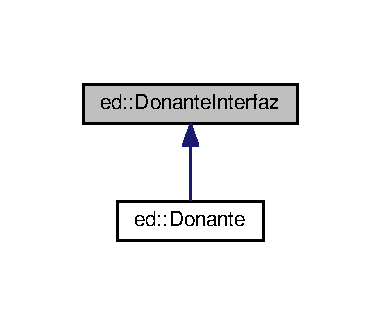
\includegraphics[width=183pt]{classed_1_1DonanteInterfaz__inherit__graph}
\end{center}
\end{figure}
\subsection*{Public Member Functions}
\begin{Indent}{\bf Observadores}\par
\begin{DoxyCompactItemize}
\item 
virtual std\+::string \hyperlink{classed_1_1DonanteInterfaz_acc116c503c26b5dee7c8982e56e5cd59}{get\+Name} () const =0
\begin{DoxyCompactList}\small\item\em Devuelve el nombre del \hyperlink{classed_1_1Donante}{Donante}. \end{DoxyCompactList}\item 
virtual std\+::string \hyperlink{classed_1_1DonanteInterfaz_ad00f542962f6585da7b465c48e65a6e9}{get\+Second\+Name} () const =0
\begin{DoxyCompactList}\small\item\em Devuelve el apellido del \hyperlink{classed_1_1Donante}{Donante}. \end{DoxyCompactList}\item 
virtual std\+::string \hyperlink{classed_1_1DonanteInterfaz_a094e88f0c9cd5c7391d5c06a09a667a1}{get\+Group} () const =0
\begin{DoxyCompactList}\small\item\em Devuelve el grupo sanguineo del donante. \end{DoxyCompactList}\item 
virtual bool \hyperlink{classed_1_1DonanteInterfaz_a3607867d874ea4fe71813acb41a0b0ef}{get\+RH} () const =0
\begin{DoxyCompactList}\small\item\em Devuelve el factor\+RH del donante. \end{DoxyCompactList}\item 
virtual int \hyperlink{classed_1_1DonanteInterfaz_a0e72966c68cab8ccb8da1c493a3a6f56}{get\+Donaciones} () const =0
\begin{DoxyCompactList}\small\item\em Devuelve el numero de donaciones realizadas por el donante. \end{DoxyCompactList}\end{DoxyCompactItemize}
\end{Indent}
\begin{Indent}{\bf Modificadores}\par
\begin{DoxyCompactItemize}
\item 
virtual void \hyperlink{classed_1_1DonanteInterfaz_a368e9dadd91e8505ea63997ec8399847}{set\+Name} (const std\+::string \&Name)=0
\begin{DoxyCompactList}\small\item\em Establece como nombre el string pasado por parametro. \end{DoxyCompactList}\item 
virtual void \hyperlink{classed_1_1DonanteInterfaz_a9f400be5262f8c75d136ea6bec7c6ee6}{set\+Second\+Name} (const std\+::string \&Second\+Name)=0
\begin{DoxyCompactList}\small\item\em Establece como apellido el string pasado por parametro. \end{DoxyCompactList}\item 
virtual void \hyperlink{classed_1_1DonanteInterfaz_a1b03ede416eb0ca704180091590d185d}{set\+Group} (const std\+::string \&Group)=0
\begin{DoxyCompactList}\small\item\em Establece como grupo Sanguineo el string pasado por parametro. \end{DoxyCompactList}\item 
virtual void \hyperlink{classed_1_1DonanteInterfaz_abca20fa89aabd5d680ed16001b48b1fb}{set\+RH} (const bool \&RH)=0
\begin{DoxyCompactList}\small\item\em Establece como apellido el string pasado por parametro. \end{DoxyCompactList}\item 
virtual void {\bfseries set\+Donaciones} (const int \&donaciones)=0\hypertarget{classed_1_1DonanteInterfaz_a7a9848b716eae64ecc9276606e7b59a3}{}\label{classed_1_1DonanteInterfaz_a7a9848b716eae64ecc9276606e7b59a3}

\end{DoxyCompactItemize}
\end{Indent}


\subsection{Detailed Description}
Clase \hyperlink{classed_1_1DonanteInterfaz}{Donante\+Interfaz} usada por \hyperlink{classed_1_1Donante}{Donante}. 

\subsection{Member Function Documentation}
\index{ed\+::\+Donante\+Interfaz@{ed\+::\+Donante\+Interfaz}!get\+Donaciones@{get\+Donaciones}}
\index{get\+Donaciones@{get\+Donaciones}!ed\+::\+Donante\+Interfaz@{ed\+::\+Donante\+Interfaz}}
\subsubsection[{\texorpdfstring{get\+Donaciones() const =0}{getDonaciones() const =0}}]{\setlength{\rightskip}{0pt plus 5cm}virtual int ed\+::\+Donante\+Interfaz\+::get\+Donaciones (
\begin{DoxyParamCaption}
{}
\end{DoxyParamCaption}
) const\hspace{0.3cm}{\ttfamily [pure virtual]}}\hypertarget{classed_1_1DonanteInterfaz_a0e72966c68cab8ccb8da1c493a3a6f56}{}\label{classed_1_1DonanteInterfaz_a0e72966c68cab8ccb8da1c493a3a6f56}


Devuelve el numero de donaciones realizadas por el donante. 

\begin{DoxyReturn}{Returns}
int 
\end{DoxyReturn}


Implemented in \hyperlink{classed_1_1Donante_ae0255405dc76a90d2ea383cd8abd4d43}{ed\+::\+Donante}.

\index{ed\+::\+Donante\+Interfaz@{ed\+::\+Donante\+Interfaz}!get\+Group@{get\+Group}}
\index{get\+Group@{get\+Group}!ed\+::\+Donante\+Interfaz@{ed\+::\+Donante\+Interfaz}}
\subsubsection[{\texorpdfstring{get\+Group() const =0}{getGroup() const =0}}]{\setlength{\rightskip}{0pt plus 5cm}virtual std\+::string ed\+::\+Donante\+Interfaz\+::get\+Group (
\begin{DoxyParamCaption}
{}
\end{DoxyParamCaption}
) const\hspace{0.3cm}{\ttfamily [pure virtual]}}\hypertarget{classed_1_1DonanteInterfaz_a094e88f0c9cd5c7391d5c06a09a667a1}{}\label{classed_1_1DonanteInterfaz_a094e88f0c9cd5c7391d5c06a09a667a1}


Devuelve el grupo sanguineo del donante. 

\begin{DoxyReturn}{Returns}
String, grupo sanguineo del donante 
\end{DoxyReturn}


Implemented in \hyperlink{classed_1_1Donante_a0b1e59193e6c887a7232d48b71bfae33}{ed\+::\+Donante}.

\index{ed\+::\+Donante\+Interfaz@{ed\+::\+Donante\+Interfaz}!get\+Name@{get\+Name}}
\index{get\+Name@{get\+Name}!ed\+::\+Donante\+Interfaz@{ed\+::\+Donante\+Interfaz}}
\subsubsection[{\texorpdfstring{get\+Name() const =0}{getName() const =0}}]{\setlength{\rightskip}{0pt plus 5cm}virtual std\+::string ed\+::\+Donante\+Interfaz\+::get\+Name (
\begin{DoxyParamCaption}
{}
\end{DoxyParamCaption}
) const\hspace{0.3cm}{\ttfamily [pure virtual]}}\hypertarget{classed_1_1DonanteInterfaz_acc116c503c26b5dee7c8982e56e5cd59}{}\label{classed_1_1DonanteInterfaz_acc116c503c26b5dee7c8982e56e5cd59}


Devuelve el nombre del \hyperlink{classed_1_1Donante}{Donante}. 

\begin{DoxyReturn}{Returns}
String, nombre del donante 
\end{DoxyReturn}


Implemented in \hyperlink{classed_1_1Donante_ae76f1220582f41d257d2f91f7addc858}{ed\+::\+Donante}.

\index{ed\+::\+Donante\+Interfaz@{ed\+::\+Donante\+Interfaz}!get\+RH@{get\+RH}}
\index{get\+RH@{get\+RH}!ed\+::\+Donante\+Interfaz@{ed\+::\+Donante\+Interfaz}}
\subsubsection[{\texorpdfstring{get\+R\+H() const =0}{getRH() const =0}}]{\setlength{\rightskip}{0pt plus 5cm}virtual bool ed\+::\+Donante\+Interfaz\+::get\+RH (
\begin{DoxyParamCaption}
{}
\end{DoxyParamCaption}
) const\hspace{0.3cm}{\ttfamily [pure virtual]}}\hypertarget{classed_1_1DonanteInterfaz_a3607867d874ea4fe71813acb41a0b0ef}{}\label{classed_1_1DonanteInterfaz_a3607867d874ea4fe71813acb41a0b0ef}


Devuelve el factor\+RH del donante. 

\begin{DoxyReturn}{Returns}
B\+O\+Ol, factor\+RH del donante 
\end{DoxyReturn}


Implemented in \hyperlink{classed_1_1Donante_aed957d321e76a3a907849d4cf0f438ee}{ed\+::\+Donante}.

\index{ed\+::\+Donante\+Interfaz@{ed\+::\+Donante\+Interfaz}!get\+Second\+Name@{get\+Second\+Name}}
\index{get\+Second\+Name@{get\+Second\+Name}!ed\+::\+Donante\+Interfaz@{ed\+::\+Donante\+Interfaz}}
\subsubsection[{\texorpdfstring{get\+Second\+Name() const =0}{getSecondName() const =0}}]{\setlength{\rightskip}{0pt plus 5cm}virtual std\+::string ed\+::\+Donante\+Interfaz\+::get\+Second\+Name (
\begin{DoxyParamCaption}
{}
\end{DoxyParamCaption}
) const\hspace{0.3cm}{\ttfamily [pure virtual]}}\hypertarget{classed_1_1DonanteInterfaz_ad00f542962f6585da7b465c48e65a6e9}{}\label{classed_1_1DonanteInterfaz_ad00f542962f6585da7b465c48e65a6e9}


Devuelve el apellido del \hyperlink{classed_1_1Donante}{Donante}. 

\begin{DoxyReturn}{Returns}
String, apellido del donante 
\end{DoxyReturn}


Implemented in \hyperlink{classed_1_1Donante_ace0406348e755517d3e80ceff18a2f59}{ed\+::\+Donante}.

\index{ed\+::\+Donante\+Interfaz@{ed\+::\+Donante\+Interfaz}!set\+Group@{set\+Group}}
\index{set\+Group@{set\+Group}!ed\+::\+Donante\+Interfaz@{ed\+::\+Donante\+Interfaz}}
\subsubsection[{\texorpdfstring{set\+Group(const std\+::string \&\+Group)=0}{setGroup(const std::string &Group)=0}}]{\setlength{\rightskip}{0pt plus 5cm}virtual void ed\+::\+Donante\+Interfaz\+::set\+Group (
\begin{DoxyParamCaption}
\item[{const std\+::string \&}]{Group}
\end{DoxyParamCaption}
)\hspace{0.3cm}{\ttfamily [pure virtual]}}\hypertarget{classed_1_1DonanteInterfaz_a1b03ede416eb0ca704180091590d185d}{}\label{classed_1_1DonanteInterfaz_a1b03ede416eb0ca704180091590d185d}


Establece como grupo Sanguineo el string pasado por parametro. 


\begin{DoxyParams}{Parameters}
{\em String} & Group \\
\hline
\end{DoxyParams}
\begin{DoxyPostcond}{Postcondition}
El donante debera de tener el grupo de la variable Group 
\end{DoxyPostcond}


Implemented in \hyperlink{classed_1_1Donante_a8e8d2ac356b88e9a83b6a3a573eb76af}{ed\+::\+Donante}.

\index{ed\+::\+Donante\+Interfaz@{ed\+::\+Donante\+Interfaz}!set\+Name@{set\+Name}}
\index{set\+Name@{set\+Name}!ed\+::\+Donante\+Interfaz@{ed\+::\+Donante\+Interfaz}}
\subsubsection[{\texorpdfstring{set\+Name(const std\+::string \&\+Name)=0}{setName(const std::string &Name)=0}}]{\setlength{\rightskip}{0pt plus 5cm}virtual void ed\+::\+Donante\+Interfaz\+::set\+Name (
\begin{DoxyParamCaption}
\item[{const std\+::string \&}]{Name}
\end{DoxyParamCaption}
)\hspace{0.3cm}{\ttfamily [pure virtual]}}\hypertarget{classed_1_1DonanteInterfaz_a368e9dadd91e8505ea63997ec8399847}{}\label{classed_1_1DonanteInterfaz_a368e9dadd91e8505ea63997ec8399847}


Establece como nombre el string pasado por parametro. 


\begin{DoxyParams}{Parameters}
{\em String} & Name \\
\hline
\end{DoxyParams}
\begin{DoxyPostcond}{Postcondition}
El donante debera de tener el nombre de la variable Name 
\end{DoxyPostcond}


Implemented in \hyperlink{classed_1_1Donante_a149c2f94803ea99ca0d322e1f54eb3e9}{ed\+::\+Donante}.

\index{ed\+::\+Donante\+Interfaz@{ed\+::\+Donante\+Interfaz}!set\+RH@{set\+RH}}
\index{set\+RH@{set\+RH}!ed\+::\+Donante\+Interfaz@{ed\+::\+Donante\+Interfaz}}
\subsubsection[{\texorpdfstring{set\+R\+H(const bool \&\+R\+H)=0}{setRH(const bool &RH)=0}}]{\setlength{\rightskip}{0pt plus 5cm}virtual void ed\+::\+Donante\+Interfaz\+::set\+RH (
\begin{DoxyParamCaption}
\item[{const bool \&}]{RH}
\end{DoxyParamCaption}
)\hspace{0.3cm}{\ttfamily [pure virtual]}}\hypertarget{classed_1_1DonanteInterfaz_abca20fa89aabd5d680ed16001b48b1fb}{}\label{classed_1_1DonanteInterfaz_abca20fa89aabd5d680ed16001b48b1fb}


Establece como apellido el string pasado por parametro. 


\begin{DoxyParams}{Parameters}
{\em String} & Second\+Name \\
\hline
\end{DoxyParams}
\begin{DoxyPostcond}{Postcondition}
El donante debera de tener el apellido de la variable Second\+Name 
\end{DoxyPostcond}


Implemented in \hyperlink{classed_1_1Donante_ae0c5eed15e7f42de44bde8405e92f598}{ed\+::\+Donante}.

\index{ed\+::\+Donante\+Interfaz@{ed\+::\+Donante\+Interfaz}!set\+Second\+Name@{set\+Second\+Name}}
\index{set\+Second\+Name@{set\+Second\+Name}!ed\+::\+Donante\+Interfaz@{ed\+::\+Donante\+Interfaz}}
\subsubsection[{\texorpdfstring{set\+Second\+Name(const std\+::string \&\+Second\+Name)=0}{setSecondName(const std::string &SecondName)=0}}]{\setlength{\rightskip}{0pt plus 5cm}virtual void ed\+::\+Donante\+Interfaz\+::set\+Second\+Name (
\begin{DoxyParamCaption}
\item[{const std\+::string \&}]{Second\+Name}
\end{DoxyParamCaption}
)\hspace{0.3cm}{\ttfamily [pure virtual]}}\hypertarget{classed_1_1DonanteInterfaz_a9f400be5262f8c75d136ea6bec7c6ee6}{}\label{classed_1_1DonanteInterfaz_a9f400be5262f8c75d136ea6bec7c6ee6}


Establece como apellido el string pasado por parametro. 


\begin{DoxyParams}{Parameters}
{\em String} & Second\+Name \\
\hline
\end{DoxyParams}
\begin{DoxyPostcond}{Postcondition}
El donante debera de tener el apellido de la variable Second\+Name 
\end{DoxyPostcond}


Implemented in \hyperlink{classed_1_1Donante_a28b1027f7ceddd66a48a5aad0ead0c43}{ed\+::\+Donante}.



The documentation for this class was generated from the following file\+:\begin{DoxyCompactItemize}
\item 
includes/\hyperlink{DonanteInterfaz_8hpp}{Donante\+Interfaz.\+hpp}\end{DoxyCompactItemize}

\hypertarget{classed_1_1Monticulo}{}\section{ed\+:\+:Monticulo Class Reference}
\label{classed_1_1Monticulo}\index{ed\+::\+Monticulo@{ed\+::\+Monticulo}}


Clase \hyperlink{classed_1_1Monticulo}{Monticulo}.  




{\ttfamily \#include $<$Monticulo.\+hpp$>$}



Inheritance diagram for ed\+:\+:Monticulo\+:\nopagebreak
\begin{figure}[H]
\begin{center}
\leavevmode
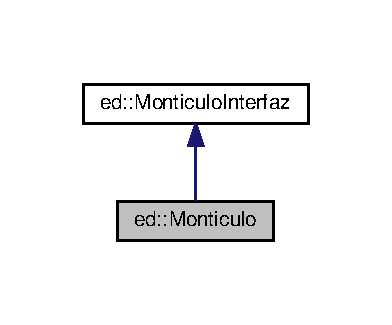
\includegraphics[width=188pt]{classed_1_1Monticulo__inherit__graph}
\end{center}
\end{figure}


Collaboration diagram for ed\+:\+:Monticulo\+:\nopagebreak
\begin{figure}[H]
\begin{center}
\leavevmode
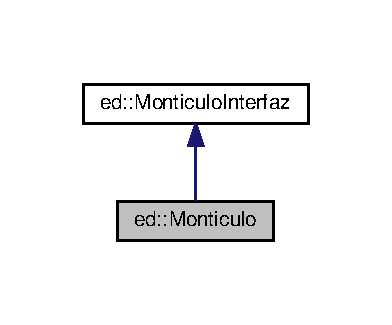
\includegraphics[width=188pt]{classed_1_1Monticulo__coll__graph}
\end{center}
\end{figure}
\subsection*{Public Member Functions}
\begin{Indent}{\bf Funciones publicas de la Clase Monticulo}\par
\begin{DoxyCompactItemize}
\item 
{\bfseries Monticulo} ()\hypertarget{classed_1_1Monticulo_a1de9bee04b411ae5f9a05f12197877ba}{}\label{classed_1_1Monticulo_a1de9bee04b411ae5f9a05f12197877ba}

\end{DoxyCompactItemize}
\end{Indent}
\begin{Indent}{\bf Observadores}\par
\begin{DoxyCompactItemize}
\item 
bool \hyperlink{classed_1_1Monticulo_ac5d5bd797bbac6fc203a70693135e07a}{empty} () const 
\begin{DoxyCompactList}\small\item\em Saber si esta vacio el montiuclo. \end{DoxyCompactList}\item 
\hyperlink{classed_1_1Donante}{Donante} \hyperlink{classed_1_1Monticulo_a0eb6ea094e966a797dc8234ec2c8d924}{cima} () const 
\begin{DoxyCompactList}\small\item\em Devuelve el donante que se encuentre en la cima. \end{DoxyCompactList}\end{DoxyCompactItemize}
\end{Indent}
\begin{Indent}{\bf Modificadores}\par
\begin{DoxyCompactItemize}
\item 
void \hyperlink{classed_1_1Monticulo_a573f0043ee88445d6b6a61d988703410}{insertar} (const \hyperlink{classed_1_1Donante}{Donante} \&d)
\begin{DoxyCompactList}\small\item\em Inserta el donante pasado por parametro. \end{DoxyCompactList}\item 
void \hyperlink{classed_1_1Monticulo_a34628b3b1210e6d4f5e240ef0e0c0a42}{delete\+Cima} ()\hypertarget{classed_1_1Monticulo_a34628b3b1210e6d4f5e240ef0e0c0a42}{}\label{classed_1_1Monticulo_a34628b3b1210e6d4f5e240ef0e0c0a42}

\begin{DoxyCompactList}\small\item\em Borrar la cima. \end{DoxyCompactList}\item 
void \hyperlink{classed_1_1Monticulo_a167e014da42bf6cb97834feb9cb26087}{borrar\+Monticulo} ()\hypertarget{classed_1_1Monticulo_a167e014da42bf6cb97834feb9cb26087}{}\label{classed_1_1Monticulo_a167e014da42bf6cb97834feb9cb26087}

\begin{DoxyCompactList}\small\item\em Eliminar el monticulo por completo. \end{DoxyCompactList}\item 
void \hyperlink{classed_1_1Monticulo_a476cdc164df729a28969054120dd7fb6}{to\+\_\+file} (std\+::string file)
\begin{DoxyCompactList}\small\item\em Salvar en un fichero el monticulo. \end{DoxyCompactList}\item 
void \hyperlink{classed_1_1Monticulo_a036c69560508db95a98ae1e666c40ca4}{cargar\+\_\+fichero} (std\+::string file)
\begin{DoxyCompactList}\small\item\em Cargar el monticulo desde un fichero. \end{DoxyCompactList}\end{DoxyCompactItemize}
\end{Indent}


\subsection{Detailed Description}
Clase \hyperlink{classed_1_1Monticulo}{Monticulo}. 

\subsection{Member Function Documentation}
\index{ed\+::\+Monticulo@{ed\+::\+Monticulo}!cargar\+\_\+fichero@{cargar\+\_\+fichero}}
\index{cargar\+\_\+fichero@{cargar\+\_\+fichero}!ed\+::\+Monticulo@{ed\+::\+Monticulo}}
\subsubsection[{\texorpdfstring{cargar\+\_\+fichero(std\+::string file)}{cargar_fichero(std::string file)}}]{\setlength{\rightskip}{0pt plus 5cm}void ed\+::\+Monticulo\+::cargar\+\_\+fichero (
\begin{DoxyParamCaption}
\item[{std\+::string}]{file}
\end{DoxyParamCaption}
)\hspace{0.3cm}{\ttfamily [inline]}}\hypertarget{classed_1_1Monticulo_a036c69560508db95a98ae1e666c40ca4}{}\label{classed_1_1Monticulo_a036c69560508db95a98ae1e666c40ca4}


Cargar el monticulo desde un fichero. 


\begin{DoxyParams}{Parameters}
{\em std\+::string} & file nombre del fichero desde el que se cargara \\
\hline
\end{DoxyParams}
\index{ed\+::\+Monticulo@{ed\+::\+Monticulo}!cima@{cima}}
\index{cima@{cima}!ed\+::\+Monticulo@{ed\+::\+Monticulo}}
\subsubsection[{\texorpdfstring{cima() const }{cima() const }}]{\setlength{\rightskip}{0pt plus 5cm}{\bf Donante} ed\+::\+Monticulo\+::cima (
\begin{DoxyParamCaption}
{}
\end{DoxyParamCaption}
) const\hspace{0.3cm}{\ttfamily [inline]}, {\ttfamily [virtual]}}\hypertarget{classed_1_1Monticulo_a0eb6ea094e966a797dc8234ec2c8d924}{}\label{classed_1_1Monticulo_a0eb6ea094e966a797dc8234ec2c8d924}


Devuelve el donante que se encuentre en la cima. 

\begin{DoxyReturn}{Returns}
\hyperlink{classed_1_1Donante}{Donante} que se encuentra en la cima 
\end{DoxyReturn}


Implements \hyperlink{classed_1_1MonticuloInterfaz_a2c30c4a9cb2f95fb14e19cca895a75b6}{ed\+::\+Monticulo\+Interfaz}.

\index{ed\+::\+Monticulo@{ed\+::\+Monticulo}!empty@{empty}}
\index{empty@{empty}!ed\+::\+Monticulo@{ed\+::\+Monticulo}}
\subsubsection[{\texorpdfstring{empty() const }{empty() const }}]{\setlength{\rightskip}{0pt plus 5cm}bool ed\+::\+Monticulo\+::empty (
\begin{DoxyParamCaption}
{}
\end{DoxyParamCaption}
) const\hspace{0.3cm}{\ttfamily [inline]}, {\ttfamily [virtual]}}\hypertarget{classed_1_1Monticulo_ac5d5bd797bbac6fc203a70693135e07a}{}\label{classed_1_1Monticulo_ac5d5bd797bbac6fc203a70693135e07a}


Saber si esta vacio el montiuclo. 

\begin{DoxyReturn}{Returns}
Devuelve true si esta vacio, false en caso contrario 
\end{DoxyReturn}


Implements \hyperlink{classed_1_1MonticuloInterfaz_a05c64243f7062b1cf9cf38813e5c1e70}{ed\+::\+Monticulo\+Interfaz}.

\index{ed\+::\+Monticulo@{ed\+::\+Monticulo}!insertar@{insertar}}
\index{insertar@{insertar}!ed\+::\+Monticulo@{ed\+::\+Monticulo}}
\subsubsection[{\texorpdfstring{insertar(const Donante \&d)}{insertar(const Donante &d)}}]{\setlength{\rightskip}{0pt plus 5cm}void ed\+::\+Monticulo\+::insertar (
\begin{DoxyParamCaption}
\item[{const {\bf Donante} \&}]{d}
\end{DoxyParamCaption}
)\hspace{0.3cm}{\ttfamily [inline]}, {\ttfamily [virtual]}}\hypertarget{classed_1_1Monticulo_a573f0043ee88445d6b6a61d988703410}{}\label{classed_1_1Monticulo_a573f0043ee88445d6b6a61d988703410}


Inserta el donante pasado por parametro. 


\begin{DoxyParams}{Parameters}
{\em const} & \hyperlink{classed_1_1Donante}{Donante}\& d \+:\hyperlink{classed_1_1Donante}{Donante} a insertar \\
\hline
\end{DoxyParams}


Implements \hyperlink{classed_1_1MonticuloInterfaz_a3800d68ce174f398a3ab0c6eca4e855f}{ed\+::\+Monticulo\+Interfaz}.

\index{ed\+::\+Monticulo@{ed\+::\+Monticulo}!to\+\_\+file@{to\+\_\+file}}
\index{to\+\_\+file@{to\+\_\+file}!ed\+::\+Monticulo@{ed\+::\+Monticulo}}
\subsubsection[{\texorpdfstring{to\+\_\+file(std\+::string file)}{to_file(std::string file)}}]{\setlength{\rightskip}{0pt plus 5cm}void ed\+::\+Monticulo\+::to\+\_\+file (
\begin{DoxyParamCaption}
\item[{std\+::string}]{file}
\end{DoxyParamCaption}
)\hspace{0.3cm}{\ttfamily [inline]}}\hypertarget{classed_1_1Monticulo_a476cdc164df729a28969054120dd7fb6}{}\label{classed_1_1Monticulo_a476cdc164df729a28969054120dd7fb6}


Salvar en un fichero el monticulo. 


\begin{DoxyParams}{Parameters}
{\em std\+::string} & file nombre del fichero donde se guardara \\
\hline
\end{DoxyParams}


The documentation for this class was generated from the following file\+:\begin{DoxyCompactItemize}
\item 
includes/\hyperlink{Monticulo_8hpp}{Monticulo.\+hpp}\end{DoxyCompactItemize}

\hypertarget{classed_1_1MonticuloInterfaz}{}\section{ed\+:\+:Monticulo\+Interfaz Class Reference}
\label{classed_1_1MonticuloInterfaz}\index{ed\+::\+Monticulo\+Interfaz@{ed\+::\+Monticulo\+Interfaz}}


Clase \hyperlink{classed_1_1MonticuloInterfaz}{Monticulo\+Interfaz}.  




{\ttfamily \#include $<$Monticulo\+Interfaz.\+hpp$>$}



Inheritance diagram for ed\+:\+:Monticulo\+Interfaz\+:\nopagebreak
\begin{figure}[H]
\begin{center}
\leavevmode
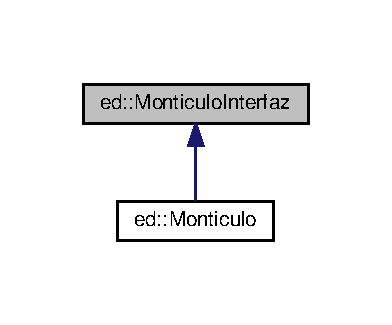
\includegraphics[width=188pt]{classed_1_1MonticuloInterfaz__inherit__graph}
\end{center}
\end{figure}
\subsection*{Public Member Functions}
\begin{Indent}{\bf Observadores}\par
\begin{DoxyCompactItemize}
\item 
virtual bool \hyperlink{classed_1_1MonticuloInterfaz_a05c64243f7062b1cf9cf38813e5c1e70}{empty} () const =0
\begin{DoxyCompactList}\small\item\em Devuelve True si no hay donantes. \end{DoxyCompactList}\item 
virtual \hyperlink{classed_1_1Donante}{Donante} \hyperlink{classed_1_1MonticuloInterfaz_a2c30c4a9cb2f95fb14e19cca895a75b6}{cima} () const =0
\begin{DoxyCompactList}\small\item\em Devuelve el donante que se encuentre en la cima. \end{DoxyCompactList}\end{DoxyCompactItemize}
\end{Indent}
\begin{Indent}{\bf Modificadores}\par
\begin{DoxyCompactItemize}
\item 
virtual void \hyperlink{classed_1_1MonticuloInterfaz_a3800d68ce174f398a3ab0c6eca4e855f}{insertar} (const \hyperlink{classed_1_1Donante}{Donante} \&d)=0
\begin{DoxyCompactList}\small\item\em Inserta un \hyperlink{classed_1_1Donante}{Donante} en el monticulo siguiendo el criterio de ordenacion. \end{DoxyCompactList}\item 
virtual void \hyperlink{classed_1_1MonticuloInterfaz_a27f0c644317d820494a28459d913bc8f}{delete\+Cima} ()=0\hypertarget{classed_1_1MonticuloInterfaz_a27f0c644317d820494a28459d913bc8f}{}\label{classed_1_1MonticuloInterfaz_a27f0c644317d820494a28459d913bc8f}

\begin{DoxyCompactList}\small\item\em Elimina el donante que se encuentre en la cima. \end{DoxyCompactList}\end{DoxyCompactItemize}
\end{Indent}


\subsection{Detailed Description}
Clase \hyperlink{classed_1_1MonticuloInterfaz}{Monticulo\+Interfaz}. 

\subsection{Member Function Documentation}
\index{ed\+::\+Monticulo\+Interfaz@{ed\+::\+Monticulo\+Interfaz}!cima@{cima}}
\index{cima@{cima}!ed\+::\+Monticulo\+Interfaz@{ed\+::\+Monticulo\+Interfaz}}
\subsubsection[{\texorpdfstring{cima() const =0}{cima() const =0}}]{\setlength{\rightskip}{0pt plus 5cm}virtual {\bf Donante} ed\+::\+Monticulo\+Interfaz\+::cima (
\begin{DoxyParamCaption}
{}
\end{DoxyParamCaption}
) const\hspace{0.3cm}{\ttfamily [pure virtual]}}\hypertarget{classed_1_1MonticuloInterfaz_a2c30c4a9cb2f95fb14e19cca895a75b6}{}\label{classed_1_1MonticuloInterfaz_a2c30c4a9cb2f95fb14e19cca895a75b6}


Devuelve el donante que se encuentre en la cima. 

\begin{DoxyReturn}{Returns}
\hyperlink{classed_1_1Donante}{Donante} 
\end{DoxyReturn}


Implemented in \hyperlink{classed_1_1Monticulo_a0eb6ea094e966a797dc8234ec2c8d924}{ed\+::\+Monticulo}.

\index{ed\+::\+Monticulo\+Interfaz@{ed\+::\+Monticulo\+Interfaz}!empty@{empty}}
\index{empty@{empty}!ed\+::\+Monticulo\+Interfaz@{ed\+::\+Monticulo\+Interfaz}}
\subsubsection[{\texorpdfstring{empty() const =0}{empty() const =0}}]{\setlength{\rightskip}{0pt plus 5cm}virtual bool ed\+::\+Monticulo\+Interfaz\+::empty (
\begin{DoxyParamCaption}
{}
\end{DoxyParamCaption}
) const\hspace{0.3cm}{\ttfamily [pure virtual]}}\hypertarget{classed_1_1MonticuloInterfaz_a05c64243f7062b1cf9cf38813e5c1e70}{}\label{classed_1_1MonticuloInterfaz_a05c64243f7062b1cf9cf38813e5c1e70}


Devuelve True si no hay donantes. 

\begin{DoxyReturn}{Returns}
Bool 
\end{DoxyReturn}


Implemented in \hyperlink{classed_1_1Monticulo_ac5d5bd797bbac6fc203a70693135e07a}{ed\+::\+Monticulo}.

\index{ed\+::\+Monticulo\+Interfaz@{ed\+::\+Monticulo\+Interfaz}!insertar@{insertar}}
\index{insertar@{insertar}!ed\+::\+Monticulo\+Interfaz@{ed\+::\+Monticulo\+Interfaz}}
\subsubsection[{\texorpdfstring{insertar(const Donante \&d)=0}{insertar(const Donante &d)=0}}]{\setlength{\rightskip}{0pt plus 5cm}virtual void ed\+::\+Monticulo\+Interfaz\+::insertar (
\begin{DoxyParamCaption}
\item[{const {\bf Donante} \&}]{d}
\end{DoxyParamCaption}
)\hspace{0.3cm}{\ttfamily [pure virtual]}}\hypertarget{classed_1_1MonticuloInterfaz_a3800d68ce174f398a3ab0c6eca4e855f}{}\label{classed_1_1MonticuloInterfaz_a3800d68ce174f398a3ab0c6eca4e855f}


Inserta un \hyperlink{classed_1_1Donante}{Donante} en el monticulo siguiendo el criterio de ordenacion. 


\begin{DoxyParams}{Parameters}
{\em \hyperlink{classed_1_1Donante}{Donante}} & d \\
\hline
\end{DoxyParams}


Implemented in \hyperlink{classed_1_1Monticulo_a573f0043ee88445d6b6a61d988703410}{ed\+::\+Monticulo}.



The documentation for this class was generated from the following file\+:\begin{DoxyCompactItemize}
\item 
includes/Monticulo\+Interfaz.\+hpp\end{DoxyCompactItemize}

\chapter{File Documentation}
\hypertarget{colors_8hpp}{}\section{includes/colors.hpp File Reference}
\label{colors_8hpp}\index{includes/colors.\+hpp@{includes/colors.\+hpp}}


Colores para la terminal.  


This graph shows which files directly or indirectly include this file\+:
\nopagebreak
\begin{figure}[H]
\begin{center}
\leavevmode
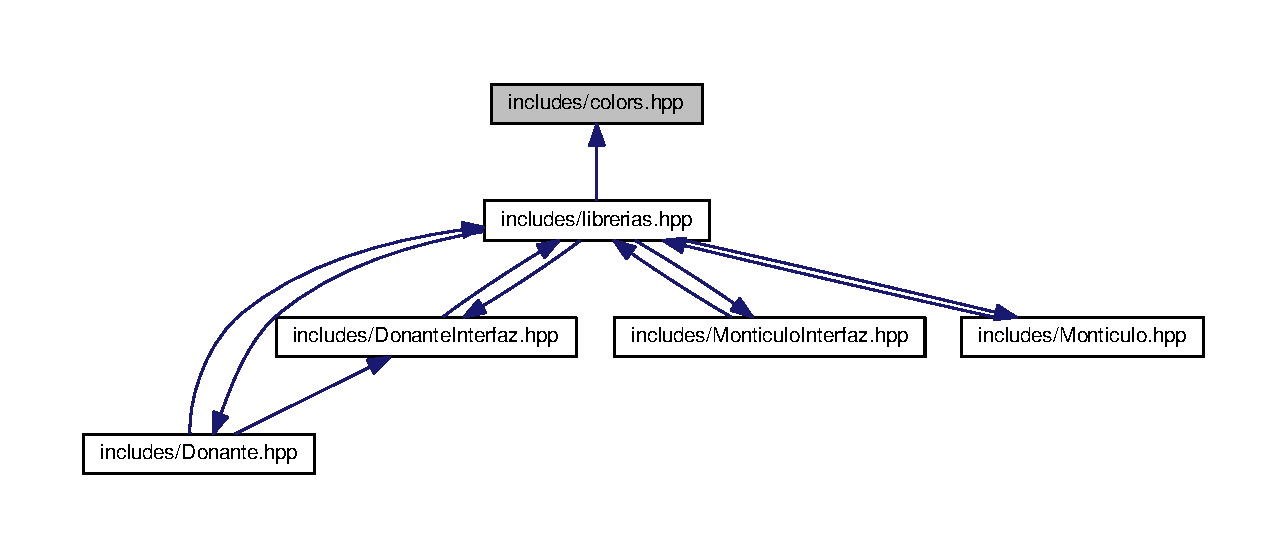
\includegraphics[width=350pt]{colors_8hpp__dep__incl}
\end{center}
\end{figure}
\subsection*{Macros}
\begin{DoxyCompactItemize}
\item 
\#define \hyperlink{colors_8hpp_abb508ea8227673f419e9fe3a86c30d8e}{F\+A\+IL}~\char`\"{}\textbackslash{}033\mbox{[}91m\char`\"{}
\item 
\#define \hyperlink{colors_8hpp_a385c3e1e3d690c32ec87a16e6422d922}{O\+K\+G\+R\+E\+EN}~\char`\"{}\textbackslash{}033\mbox{[}92m\char`\"{}
\item 
\#define \hyperlink{colors_8hpp_a5cb439d9f933fde4cf23caa370c030e7}{W\+A\+R\+N\+I\+NG}~\char`\"{}\textbackslash{}033\mbox{[}93m\char`\"{}
\item 
\#define \hyperlink{colors_8hpp_ad9f51d85a4d6d80cd00f6a3461bb183f}{O\+K\+B\+L\+UE}~\char`\"{}\textbackslash{}033\mbox{[}94m\char`\"{}
\item 
\#define \hyperlink{colors_8hpp_ab7770a7f0d95e67620ff6ed347a07a56}{H\+E\+A\+D\+ER}~\char`\"{}\textbackslash{}033\mbox{[}95m\char`\"{}
\item 
\#define \hyperlink{colors_8hpp_ac9e7df060e19345a81e30a747f8a2d99}{E\+N\+DC}~\char`\"{}\textbackslash{}033\mbox{[}0m\char`\"{}
\end{DoxyCompactItemize}


\subsection{Detailed Description}
Colores para la terminal. 

\begin{DoxyAuthor}{Author}
Jose Manuel Marquez Matarin 
\end{DoxyAuthor}


\subsection{Macro Definition Documentation}
\index{colors.\+hpp@{colors.\+hpp}!E\+N\+DC@{E\+N\+DC}}
\index{E\+N\+DC@{E\+N\+DC}!colors.\+hpp@{colors.\+hpp}}
\subsubsection[{\texorpdfstring{E\+N\+DC}{ENDC}}]{\setlength{\rightskip}{0pt plus 5cm}\#define E\+N\+DC~\char`\"{}\textbackslash{}033\mbox{[}0m\char`\"{}}\hypertarget{colors_8hpp_ac9e7df060e19345a81e30a747f8a2d99}{}\label{colors_8hpp_ac9e7df060e19345a81e30a747f8a2d99}
E\+ND color. \index{colors.\+hpp@{colors.\+hpp}!F\+A\+IL@{F\+A\+IL}}
\index{F\+A\+IL@{F\+A\+IL}!colors.\+hpp@{colors.\+hpp}}
\subsubsection[{\texorpdfstring{F\+A\+IL}{FAIL}}]{\setlength{\rightskip}{0pt plus 5cm}\#define F\+A\+IL~\char`\"{}\textbackslash{}033\mbox{[}91m\char`\"{}}\hypertarget{colors_8hpp_abb508ea8227673f419e9fe3a86c30d8e}{}\label{colors_8hpp_abb508ea8227673f419e9fe3a86c30d8e}
Color red. \index{colors.\+hpp@{colors.\+hpp}!H\+E\+A\+D\+ER@{H\+E\+A\+D\+ER}}
\index{H\+E\+A\+D\+ER@{H\+E\+A\+D\+ER}!colors.\+hpp@{colors.\+hpp}}
\subsubsection[{\texorpdfstring{H\+E\+A\+D\+ER}{HEADER}}]{\setlength{\rightskip}{0pt plus 5cm}\#define H\+E\+A\+D\+ER~\char`\"{}\textbackslash{}033\mbox{[}95m\char`\"{}}\hypertarget{colors_8hpp_ab7770a7f0d95e67620ff6ed347a07a56}{}\label{colors_8hpp_ab7770a7f0d95e67620ff6ed347a07a56}
Color purple. \index{colors.\+hpp@{colors.\+hpp}!O\+K\+B\+L\+UE@{O\+K\+B\+L\+UE}}
\index{O\+K\+B\+L\+UE@{O\+K\+B\+L\+UE}!colors.\+hpp@{colors.\+hpp}}
\subsubsection[{\texorpdfstring{O\+K\+B\+L\+UE}{OKBLUE}}]{\setlength{\rightskip}{0pt plus 5cm}\#define O\+K\+B\+L\+UE~\char`\"{}\textbackslash{}033\mbox{[}94m\char`\"{}}\hypertarget{colors_8hpp_ad9f51d85a4d6d80cd00f6a3461bb183f}{}\label{colors_8hpp_ad9f51d85a4d6d80cd00f6a3461bb183f}
Color blue. \index{colors.\+hpp@{colors.\+hpp}!O\+K\+G\+R\+E\+EN@{O\+K\+G\+R\+E\+EN}}
\index{O\+K\+G\+R\+E\+EN@{O\+K\+G\+R\+E\+EN}!colors.\+hpp@{colors.\+hpp}}
\subsubsection[{\texorpdfstring{O\+K\+G\+R\+E\+EN}{OKGREEN}}]{\setlength{\rightskip}{0pt plus 5cm}\#define O\+K\+G\+R\+E\+EN~\char`\"{}\textbackslash{}033\mbox{[}92m\char`\"{}}\hypertarget{colors_8hpp_a385c3e1e3d690c32ec87a16e6422d922}{}\label{colors_8hpp_a385c3e1e3d690c32ec87a16e6422d922}
Color green. \index{colors.\+hpp@{colors.\+hpp}!W\+A\+R\+N\+I\+NG@{W\+A\+R\+N\+I\+NG}}
\index{W\+A\+R\+N\+I\+NG@{W\+A\+R\+N\+I\+NG}!colors.\+hpp@{colors.\+hpp}}
\subsubsection[{\texorpdfstring{W\+A\+R\+N\+I\+NG}{WARNING}}]{\setlength{\rightskip}{0pt plus 5cm}\#define W\+A\+R\+N\+I\+NG~\char`\"{}\textbackslash{}033\mbox{[}93m\char`\"{}}\hypertarget{colors_8hpp_a5cb439d9f933fde4cf23caa370c030e7}{}\label{colors_8hpp_a5cb439d9f933fde4cf23caa370c030e7}
Color yellow. 
\hypertarget{Donante_8hpp}{}\section{includes/\+Donante.hpp File Reference}
\label{Donante_8hpp}\index{includes/\+Donante.\+hpp@{includes/\+Donante.\+hpp}}


Clase Donante, hereda de Donante\+Interfaz.  


{\ttfamily \#include \char`\"{}librerias.\+hpp\char`\"{}}\\*
{\ttfamily \#include \char`\"{}Donante\+Interfaz.\+hpp\char`\"{}}\\*
Include dependency graph for Donante.\+hpp\+:
\nopagebreak
\begin{figure}[H]
\begin{center}
\leavevmode
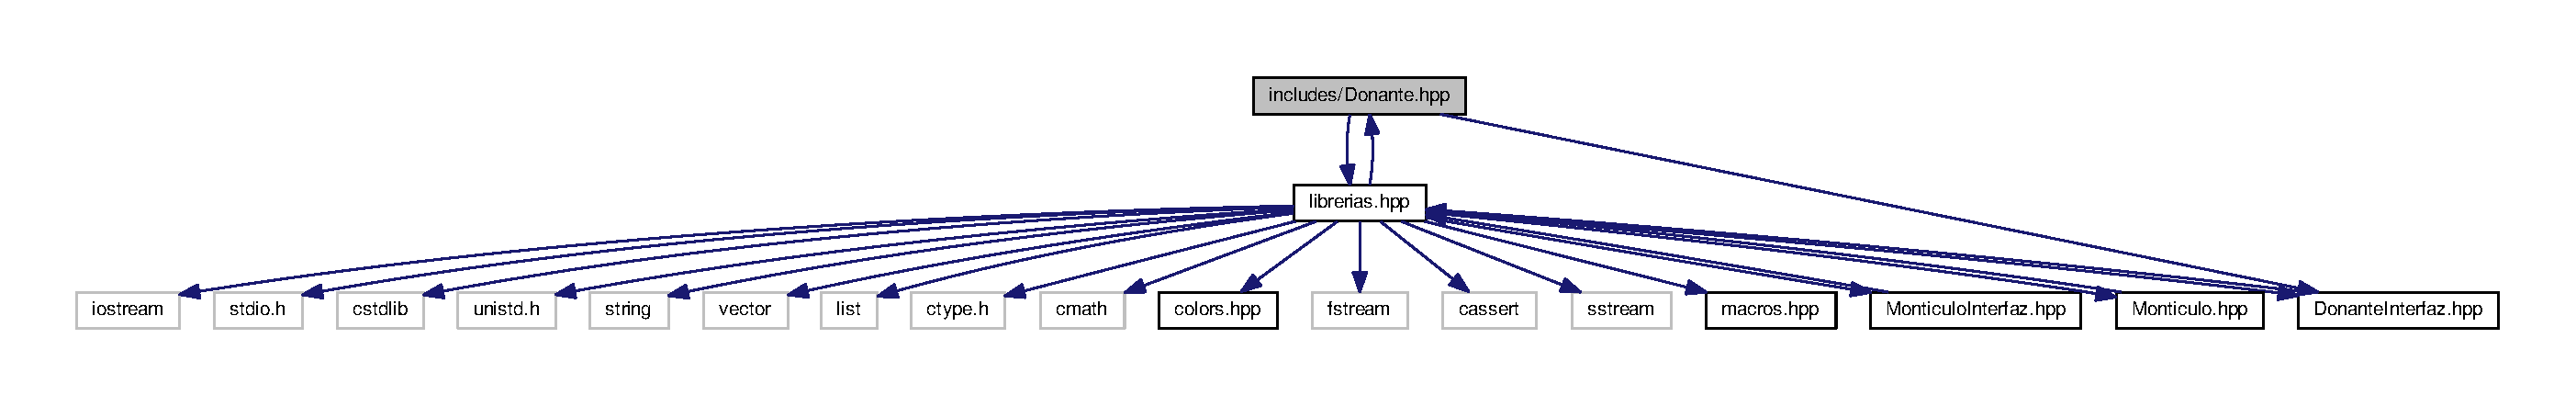
\includegraphics[width=350pt]{Donante_8hpp__incl}
\end{center}
\end{figure}
This graph shows which files directly or indirectly include this file\+:\nopagebreak
\begin{figure}[H]
\begin{center}
\leavevmode
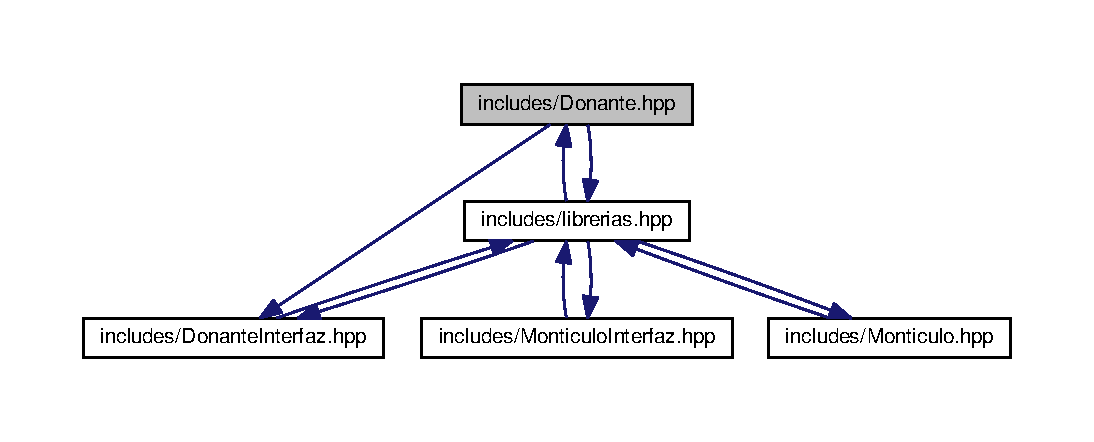
\includegraphics[width=350pt]{Donante_8hpp__dep__incl}
\end{center}
\end{figure}
\subsection*{Classes}
\begin{DoxyCompactItemize}
\item 
class \hyperlink{classed_1_1Donante}{ed\+::\+Donante}
\begin{DoxyCompactList}\small\item\em Clase \hyperlink{classed_1_1Donante}{Donante}. \end{DoxyCompactList}\end{DoxyCompactItemize}
\subsection*{Namespaces}
\begin{DoxyCompactItemize}
\item 
 \hyperlink{namespaceed}{ed}
\begin{DoxyCompactList}\small\item\em Espacio de nombres ED. \end{DoxyCompactList}\end{DoxyCompactItemize}


\subsection{Detailed Description}
Clase Donante, hereda de Donante\+Interfaz. 

\begin{DoxyAuthor}{Author}
Jose Manuel Marquez Matarin 
\end{DoxyAuthor}

\hypertarget{DonanteInterfaz_8hpp}{}\section{includes/\+Donante\+Interfaz.hpp File Reference}
\label{DonanteInterfaz_8hpp}\index{includes/\+Donante\+Interfaz.\+hpp@{includes/\+Donante\+Interfaz.\+hpp}}


Interfaz de la clase donante.  


{\ttfamily \#include \char`\"{}librerias.\+hpp\char`\"{}}\\*
Include dependency graph for Donante\+Interfaz.\+hpp\+:
\nopagebreak
\begin{figure}[H]
\begin{center}
\leavevmode
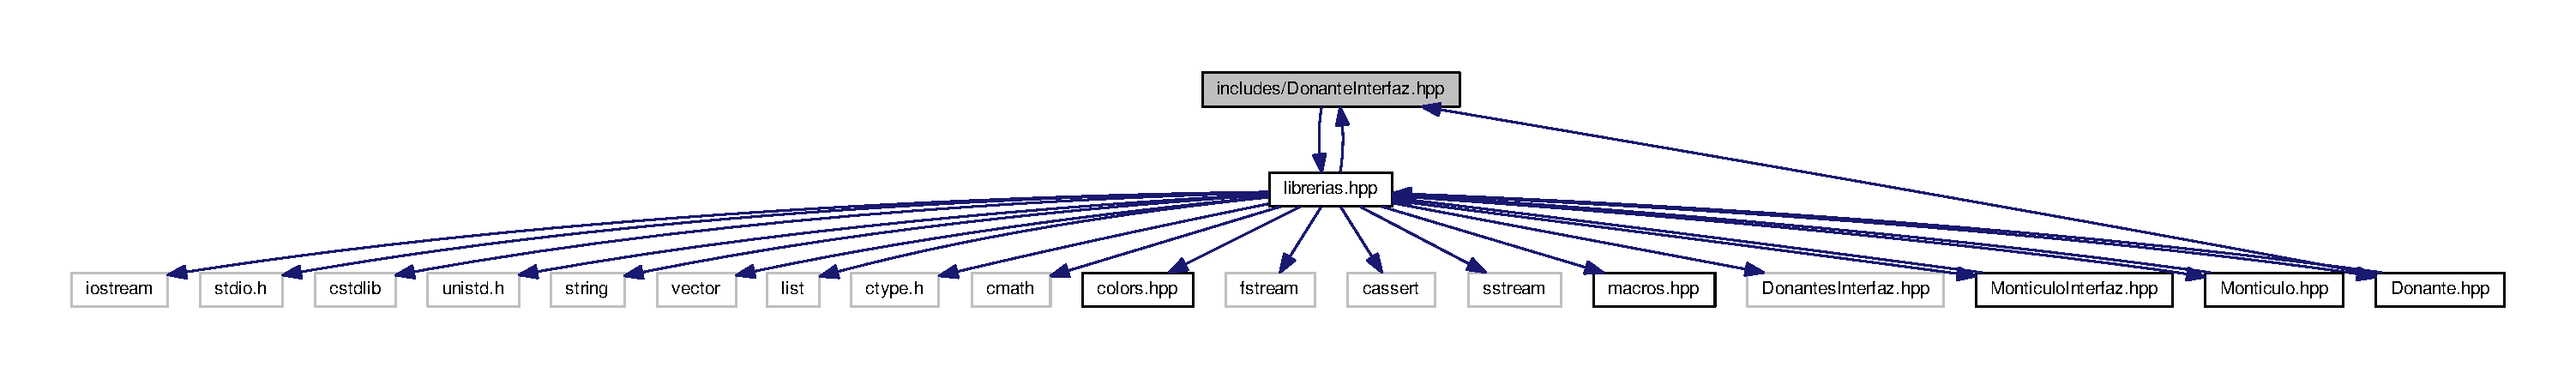
\includegraphics[width=350pt]{DonanteInterfaz_8hpp__incl}
\end{center}
\end{figure}
This graph shows which files directly or indirectly include this file\+:
\nopagebreak
\begin{figure}[H]
\begin{center}
\leavevmode
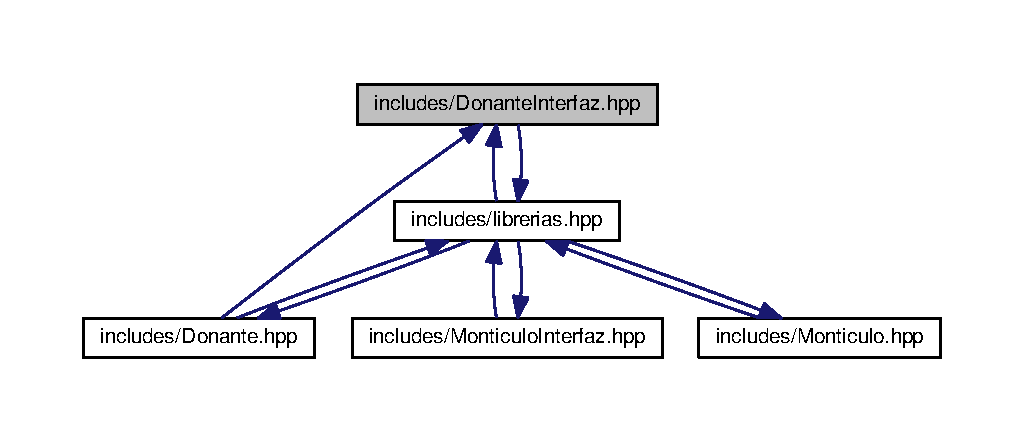
\includegraphics[width=350pt]{DonanteInterfaz_8hpp__dep__incl}
\end{center}
\end{figure}
\subsection*{Classes}
\begin{DoxyCompactItemize}
\item 
class \hyperlink{classed_1_1DonanteInterfaz}{ed\+::\+Donante\+Interfaz}
\begin{DoxyCompactList}\small\item\em Clase \hyperlink{classed_1_1DonanteInterfaz}{Donante\+Interfaz} usada por \hyperlink{classed_1_1Donante}{Donante}. \end{DoxyCompactList}\end{DoxyCompactItemize}
\subsection*{Namespaces}
\begin{DoxyCompactItemize}
\item 
 \hyperlink{namespaceed}{ed}
\begin{DoxyCompactList}\small\item\em Espacio de nombres ED. \end{DoxyCompactList}\end{DoxyCompactItemize}


\subsection{Detailed Description}
Interfaz de la clase donante. 

\begin{DoxyAuthor}{Author}
Jose Manuel Marquez Matarin 
\end{DoxyAuthor}

\hypertarget{librerias_8hpp}{}\section{includes/librerias.hpp File Reference}
\label{librerias_8hpp}\index{includes/librerias.\+hpp@{includes/librerias.\+hpp}}


Librerias incluidas en los hpp.  


{\ttfamily \#include $<$iostream$>$}\\*
{\ttfamily \#include $<$stdio.\+h$>$}\\*
{\ttfamily \#include $<$cstdlib$>$}\\*
{\ttfamily \#include $<$unistd.\+h$>$}\\*
{\ttfamily \#include $<$string$>$}\\*
{\ttfamily \#include $<$vector$>$}\\*
{\ttfamily \#include $<$list$>$}\\*
{\ttfamily \#include $<$ctype.\+h$>$}\\*
{\ttfamily \#include $<$cmath$>$}\\*
{\ttfamily \#include \char`\"{}colors.\+hpp\char`\"{}}\\*
{\ttfamily \#include $<$fstream$>$}\\*
{\ttfamily \#include $<$cassert$>$}\\*
{\ttfamily \#include $<$sstream$>$}\\*
{\ttfamily \#include \char`\"{}macros.\+hpp\char`\"{}}\\*
{\ttfamily \#include \char`\"{}Donante.\+hpp\char`\"{}}\\*
{\ttfamily \#include \char`\"{}Donantes\+Interfaz.\+hpp\char`\"{}}\\*
{\ttfamily \#include \char`\"{}Donante\+Interfaz.\+hpp\char`\"{}}\\*
{\ttfamily \#include \char`\"{}Monticulo\+Interfaz.\+hpp\char`\"{}}\\*
{\ttfamily \#include \char`\"{}Monticulo.\+hpp\char`\"{}}\\*
Include dependency graph for librerias.\+hpp\+:
\nopagebreak
\begin{figure}[H]
\begin{center}
\leavevmode
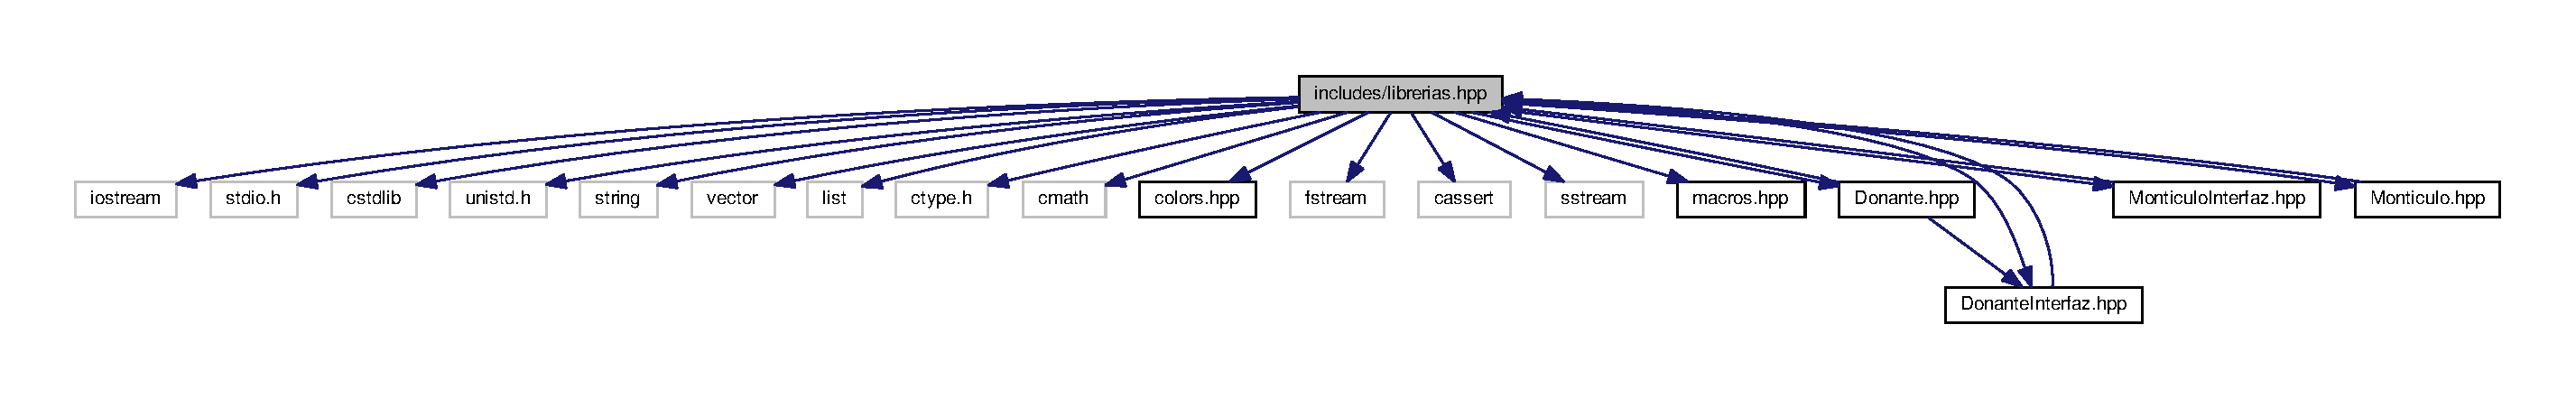
\includegraphics[width=350pt]{librerias_8hpp__incl}
\end{center}
\end{figure}
This graph shows which files directly or indirectly include this file\+:
\nopagebreak
\begin{figure}[H]
\begin{center}
\leavevmode
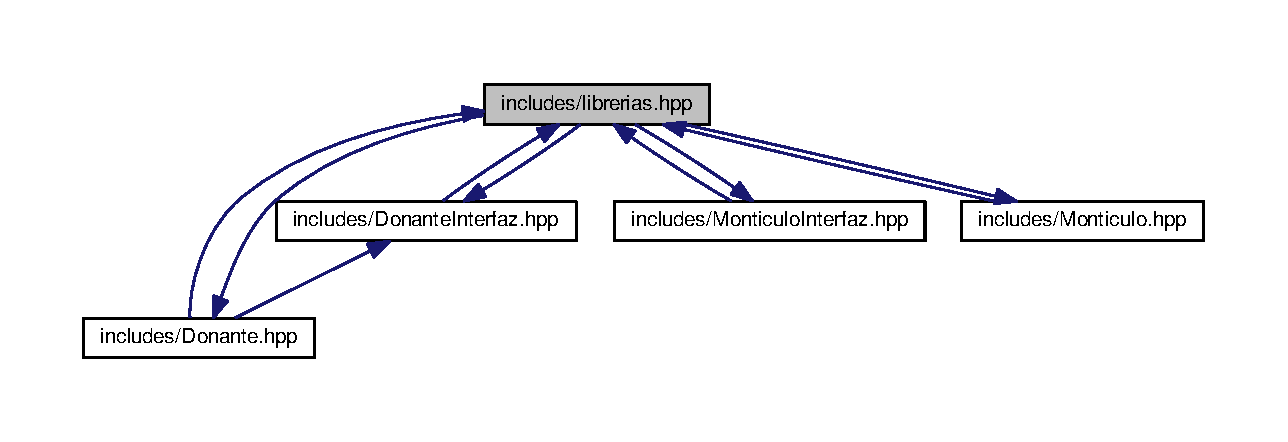
\includegraphics[width=350pt]{librerias_8hpp__dep__incl}
\end{center}
\end{figure}


\subsection{Detailed Description}
Librerias incluidas en los hpp. 

\begin{DoxyAuthor}{Author}
Jose Manuel Marquez Matarin 
\end{DoxyAuthor}

\hypertarget{macros_8hpp}{}\section{includes/macros.hpp File Reference}
\label{macros_8hpp}\index{includes/macros.\+hpp@{includes/macros.\+hpp}}


Macros para el diseño de pantallas.  


This graph shows which files directly or indirectly include this file\+:
\nopagebreak
\begin{figure}[H]
\begin{center}
\leavevmode
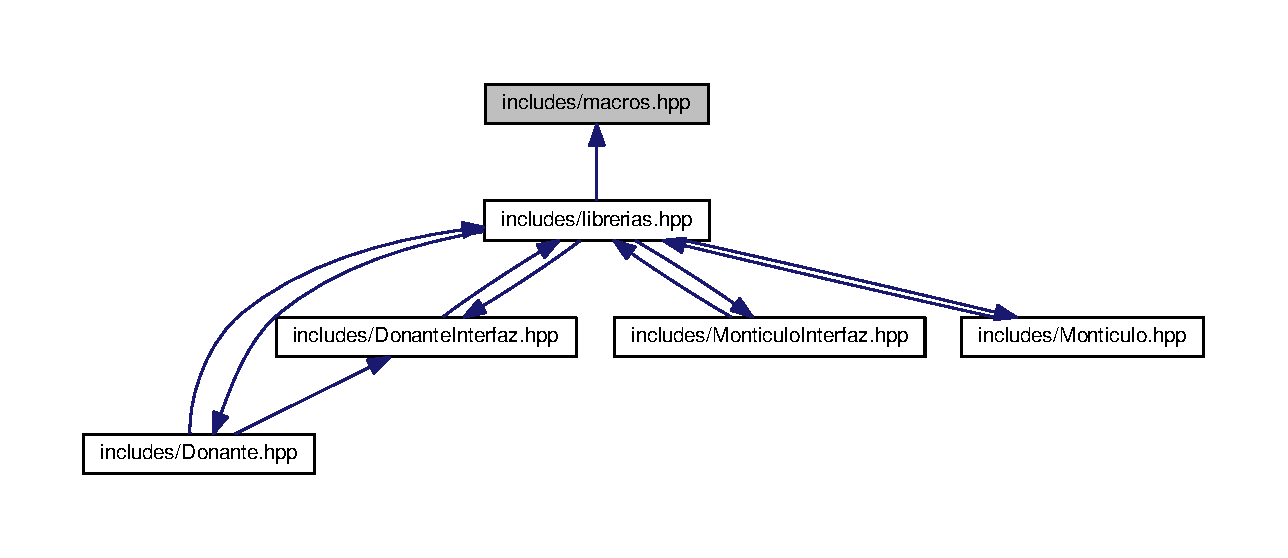
\includegraphics[width=350pt]{macros_8hpp__dep__incl}
\end{center}
\end{figure}
\subsection*{Macros}
\begin{DoxyCompactItemize}
\item 
\#define \hyperlink{macros_8hpp_a1e26748f72802cc32341cc3846db931f}{L\+U\+G\+AR}(x,  y)~printf(\char`\"{}\textbackslash{}033\mbox{[}\%d;\%dH\char`\"{}, x, y)
\item 
\#define \hyperlink{macros_8hpp_a79bf316fce01e63d76dddcdcbe72ab1c}{B\+O\+R\+R\+AR}~printf(\char`\"{}\textbackslash{}33\mbox{[}2\+J\char`\"{})
\item 
\#define \hyperlink{macros_8hpp_ab86c2fc65d2b4c5205910f548828dcb9}{P\+A\+R\+P\+A\+D\+EO}~printf(\char`\"{}\%c\mbox{[}5m\char`\"{}, 27)
\item 
\#define \hyperlink{macros_8hpp_af2815fb445b50124864e3f2f958fac24}{A\+P\+A\+GA}~printf(\char`\"{}\%c\mbox{[}0m\char`\"{}, 27)
\item 
\#define \hyperlink{macros_8hpp_ac6cb5eae7b643f5d13c9d546e81dbcaf}{I\+N\+V\+E\+R\+SO}~printf(\char`\"{}\%c\mbox{[}7m\char`\"{}, 27)
\item 
\#define \hyperlink{macros_8hpp_a3ab8b4157fd29a2336c702b26a967bb9}{S\+U\+B\+R\+A\+Y\+A\+DO}~printf(\char`\"{}\%c\mbox{[}4m\char`\"{}, 27)
\item 
\#define \hyperlink{macros_8hpp_af7eea73aeb56d77e1d56471ab214f8e2}{I\+N\+T\+E\+N\+S\+I\+D\+AD}~printf(\char`\"{}\%c\mbox{[}1m\char`\"{}, 27)
\end{DoxyCompactItemize}


\subsection{Detailed Description}
Macros para el diseño de pantallas. 



\subsection{Macro Definition Documentation}
\index{macros.\+hpp@{macros.\+hpp}!A\+P\+A\+GA@{A\+P\+A\+GA}}
\index{A\+P\+A\+GA@{A\+P\+A\+GA}!macros.\+hpp@{macros.\+hpp}}
\subsubsection[{\texorpdfstring{A\+P\+A\+GA}{APAGA}}]{\setlength{\rightskip}{0pt plus 5cm}\#define A\+P\+A\+GA~printf(\char`\"{}\%c\mbox{[}0m\char`\"{}, 27)}\hypertarget{macros_8hpp_af2815fb445b50124864e3f2f958fac24}{}\label{macros_8hpp_af2815fb445b50124864e3f2f958fac24}
Macro of interaction. \index{macros.\+hpp@{macros.\+hpp}!B\+O\+R\+R\+AR@{B\+O\+R\+R\+AR}}
\index{B\+O\+R\+R\+AR@{B\+O\+R\+R\+AR}!macros.\+hpp@{macros.\+hpp}}
\subsubsection[{\texorpdfstring{B\+O\+R\+R\+AR}{BORRAR}}]{\setlength{\rightskip}{0pt plus 5cm}\#define B\+O\+R\+R\+AR~printf(\char`\"{}\textbackslash{}33\mbox{[}2\+J\char`\"{})}\hypertarget{macros_8hpp_a79bf316fce01e63d76dddcdcbe72ab1c}{}\label{macros_8hpp_a79bf316fce01e63d76dddcdcbe72ab1c}
Macro for delete. \index{macros.\+hpp@{macros.\+hpp}!I\+N\+T\+E\+N\+S\+I\+D\+AD@{I\+N\+T\+E\+N\+S\+I\+D\+AD}}
\index{I\+N\+T\+E\+N\+S\+I\+D\+AD@{I\+N\+T\+E\+N\+S\+I\+D\+AD}!macros.\+hpp@{macros.\+hpp}}
\subsubsection[{\texorpdfstring{I\+N\+T\+E\+N\+S\+I\+D\+AD}{INTENSIDAD}}]{\setlength{\rightskip}{0pt plus 5cm}\#define I\+N\+T\+E\+N\+S\+I\+D\+AD~printf(\char`\"{}\%c\mbox{[}1m\char`\"{}, 27)}\hypertarget{macros_8hpp_af7eea73aeb56d77e1d56471ab214f8e2}{}\label{macros_8hpp_af7eea73aeb56d77e1d56471ab214f8e2}
Macro of interaction. \index{macros.\+hpp@{macros.\+hpp}!I\+N\+V\+E\+R\+SO@{I\+N\+V\+E\+R\+SO}}
\index{I\+N\+V\+E\+R\+SO@{I\+N\+V\+E\+R\+SO}!macros.\+hpp@{macros.\+hpp}}
\subsubsection[{\texorpdfstring{I\+N\+V\+E\+R\+SO}{INVERSO}}]{\setlength{\rightskip}{0pt plus 5cm}\#define I\+N\+V\+E\+R\+SO~printf(\char`\"{}\%c\mbox{[}7m\char`\"{}, 27)}\hypertarget{macros_8hpp_ac6cb5eae7b643f5d13c9d546e81dbcaf}{}\label{macros_8hpp_ac6cb5eae7b643f5d13c9d546e81dbcaf}
Macro of interaction. \index{macros.\+hpp@{macros.\+hpp}!L\+U\+G\+AR@{L\+U\+G\+AR}}
\index{L\+U\+G\+AR@{L\+U\+G\+AR}!macros.\+hpp@{macros.\+hpp}}
\subsubsection[{\texorpdfstring{L\+U\+G\+AR}{LUGAR}}]{\setlength{\rightskip}{0pt plus 5cm}\#define L\+U\+G\+AR(
\begin{DoxyParamCaption}
\item[{}]{x, }
\item[{}]{y}
\end{DoxyParamCaption}
)~printf(\char`\"{}\textbackslash{}033\mbox{[}\%d;\%dH\char`\"{}, x, y)}\hypertarget{macros_8hpp_a1e26748f72802cc32341cc3846db931f}{}\label{macros_8hpp_a1e26748f72802cc32341cc3846db931f}
Macro for place. \index{macros.\+hpp@{macros.\+hpp}!P\+A\+R\+P\+A\+D\+EO@{P\+A\+R\+P\+A\+D\+EO}}
\index{P\+A\+R\+P\+A\+D\+EO@{P\+A\+R\+P\+A\+D\+EO}!macros.\+hpp@{macros.\+hpp}}
\subsubsection[{\texorpdfstring{P\+A\+R\+P\+A\+D\+EO}{PARPADEO}}]{\setlength{\rightskip}{0pt plus 5cm}\#define P\+A\+R\+P\+A\+D\+EO~printf(\char`\"{}\%c\mbox{[}5m\char`\"{}, 27)}\hypertarget{macros_8hpp_ab86c2fc65d2b4c5205910f548828dcb9}{}\label{macros_8hpp_ab86c2fc65d2b4c5205910f548828dcb9}
Macro of interaction. \index{macros.\+hpp@{macros.\+hpp}!S\+U\+B\+R\+A\+Y\+A\+DO@{S\+U\+B\+R\+A\+Y\+A\+DO}}
\index{S\+U\+B\+R\+A\+Y\+A\+DO@{S\+U\+B\+R\+A\+Y\+A\+DO}!macros.\+hpp@{macros.\+hpp}}
\subsubsection[{\texorpdfstring{S\+U\+B\+R\+A\+Y\+A\+DO}{SUBRAYADO}}]{\setlength{\rightskip}{0pt plus 5cm}\#define S\+U\+B\+R\+A\+Y\+A\+DO~printf(\char`\"{}\%c\mbox{[}4m\char`\"{}, 27)}\hypertarget{macros_8hpp_a3ab8b4157fd29a2336c702b26a967bb9}{}\label{macros_8hpp_a3ab8b4157fd29a2336c702b26a967bb9}
Macro of interaction. 
\hypertarget{Monticulo_8hpp}{}\section{includes/\+Monticulo.hpp File Reference}
\label{Monticulo_8hpp}\index{includes/\+Monticulo.\+hpp@{includes/\+Monticulo.\+hpp}}


Clase Monticulo, hereda de Monticulo\+Interfaz.  


{\ttfamily \#include \char`\"{}librerias.\+hpp\char`\"{}}\\*
Include dependency graph for Monticulo.\+hpp\+:
\nopagebreak
\begin{figure}[H]
\begin{center}
\leavevmode
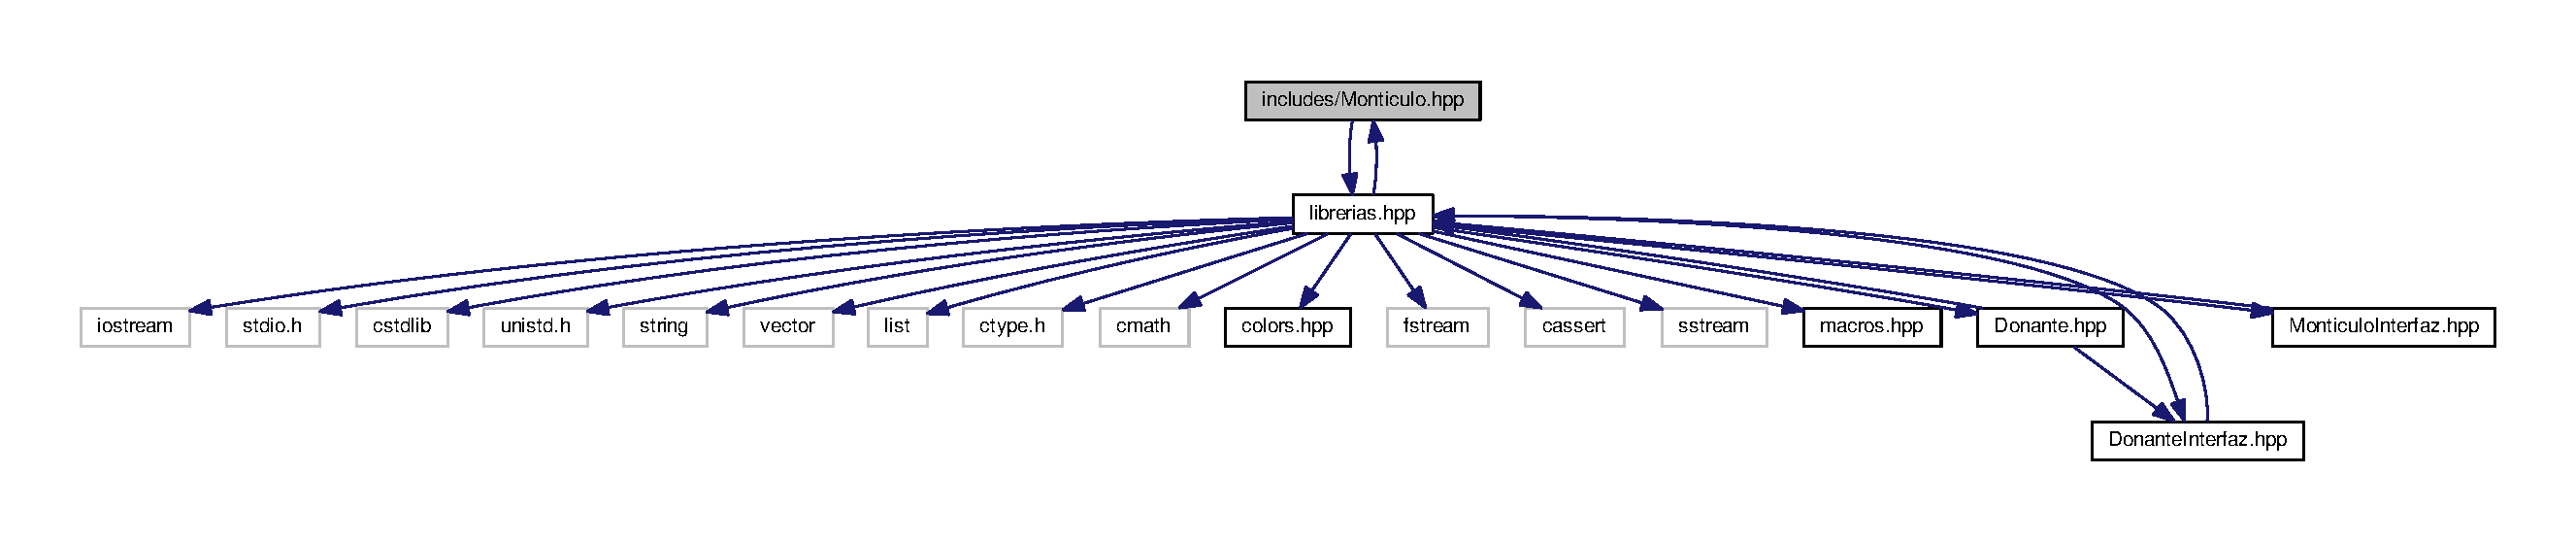
\includegraphics[width=350pt]{Monticulo_8hpp__incl}
\end{center}
\end{figure}
This graph shows which files directly or indirectly include this file\+:\nopagebreak
\begin{figure}[H]
\begin{center}
\leavevmode
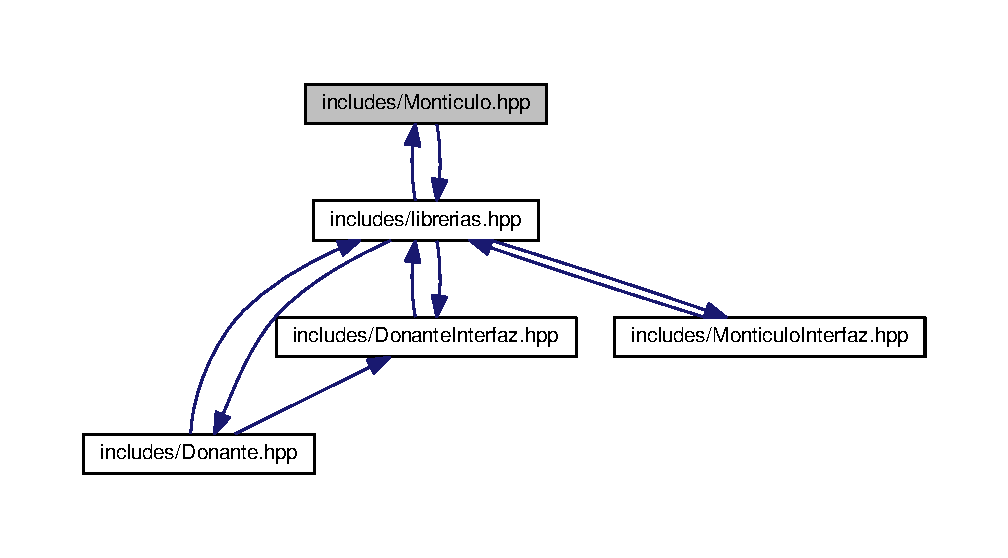
\includegraphics[width=350pt]{Monticulo_8hpp__dep__incl}
\end{center}
\end{figure}
\subsection*{Classes}
\begin{DoxyCompactItemize}
\item 
class \hyperlink{classed_1_1Monticulo}{ed\+::\+Monticulo}
\begin{DoxyCompactList}\small\item\em Clase \hyperlink{classed_1_1Monticulo}{Monticulo}. \end{DoxyCompactList}\end{DoxyCompactItemize}
\subsection*{Namespaces}
\begin{DoxyCompactItemize}
\item 
 \hyperlink{namespaceed}{ed}
\begin{DoxyCompactList}\small\item\em Espacio de nombres ED. \end{DoxyCompactList}\end{DoxyCompactItemize}


\subsection{Detailed Description}
Clase Monticulo, hereda de Monticulo\+Interfaz. 

\begin{DoxyAuthor}{Author}
Jose Manuel Marquez Matarin 
\end{DoxyAuthor}

%--- End generated contents ---

% Index
\backmatter
\newpage
\phantomsection
\clearemptydoublepage
\addcontentsline{toc}{chapter}{Index}
\printindex

\end{document}
